\documentclass[11pt,titlepage]{article}
\usepackage{amsmath}
\usepackage[hmargin=30mm, vmargin=30mm]{geometry}
\usepackage{bm}
\usepackage[makeroom]{cancel}
\usepackage{graphicx}
\usepackage[colorlinks=true, linkcolor=blue, urlcolor=blue]{hyperref}
\hypersetup{pdfnewwindow=true}
\usepackage{titlepic}
\usepackage[usenames, dvipsnames]{color}
\renewcommand{\contentsname}{What's on the Docket?\\{\small (I promise the rest of the book is far more fun than this boring Table of Contents)}}
\usepackage{amsthm}
\newtheorem{thm}{Theorem}
\usepackage{amssymb}
\usepackage{wrapfig}
\usepackage{gensymb}
\usepackage{sidecap}
\usepackage{mwe}
\usepackage{tikz}
\usepackage{comment}
\usepackage{relsize}
\usepackage{color}
\usepackage{pgfplots}
\usepackage{caption}
\allowdisplaybreaks
%\usepackage[bottom]{footmisc}

\graphicspath{{./Images/}}
\title{An Introduction to Pi ($\pi$)\vspace{-0.5cm}}
\author{Matthew Jordan}
\date{\today\vspace{2cm}\begin{center}
\includegraphics[scale=1.2]{Pi}
\end{center}}

\begin{document}

\maketitle
\begin{comment}
\section*{Preface}

Hi there! First off, let me just say that I am exceptionally flattered that you have decided to read this ol' thang. I really appreciate that you've even made it this far. I'm not sure what it would best be called -- book? article? magnum opus? -- but these musings are my first foray into writing about math, a pursuit I hope to continue for at least a lifetime.

There are a few important things I figure I ought to mention before we get this thing going. First off, I haven't really written for any specific audience here. Admittedly, there are some parts of this book (especially in the second half) that will unquestionably baffle folks who haven't taken some university level math. But don't let potentially intimidating symbols deter you from reading this in full; the historical content and mathematical intuition are totally accessible. I've made a very conscientious effort to use very little technical language, often at the expense of brevity. But I think that being understood is far more important than being concise, so hopefully what I lack in terseness I make up for in clarity. 

Second, you'll very quickly notice that I'm not an expert in graphic design, nor am I particularly skilled at making things look pretty. Fortunately, \LaTeX (the program that makes math look beautiful) does most of the formatting for me. That being said, I'm really just getting started on \LaTeX, so I still have much to learn and would love love love any advice on how to improve.

Third, I should probably talk a bit about references. I admittedly haven't been all that careful with references and citations here. Most of the information can be found (and is properly sourced) on Wikipedia or Wolfram, and I promise it's all legit. Perhaps in the second edition I'll have a bibliography. In the interest of humour I have bended some historical information, but none of the math has been modified for comedic purposes. 

Finally, I want to thank a few people who helped me out with this project. The whole inspiration for this came from David Laing, who at the beginning of the summer of 2014 asked me to teach him any topics in math of my choosing. I decided that $\pi$ would be a fun subject, and figured it would be a good idea to write everything down so I wouldn't forget it, and now here we are! So thank you, David, for giving me the opportunity to teach a subject of my own choosing to a very receptive audience. 

I'm also quite indebted to Dr. Greg Moore, who taught my History of Math course and who was the first to show me how much more there is to math than the equations we learn in class. 

Shout out to Jaime Knoch \textcolor{red}{OTHER NAMES} who took the time to help me edit. I would be foolish to think that I could write this whole thing without some help, and I'm happy to say that these are some of the smartest and most helpful folks I've ever come across. Thanks for all the late night shenanigans and giggles. Despite this, there are probably finicky mistakes that have gone unnoticed, and do not hesitate to alert me if you notice anything gone awry!

Of course, as always, I need to thank the two all-time great people who have inspired me with just about everything I do: Charles Babbage and Kanye West, you guys rock. 
\\ \\
\indent
Anyway, that's enough from me. Now it's time to dust off your spectacles, sharpen your quill, and massage that noggin, because it's learning time. Let's get started! 
\\ \\
-- Matthew Jordan, September 2014  

\newpage 

\tableofcontents

\newpage
\end{comment}
\begin{center}
{\huge An Introduction to $\pi$ (Sneak Preview!)}
\end{center}
\subsection*{\label{preview}\textcolor{Plum}{Like most sneak previews, I'm going to pick up somewhere totally random and leave you utterly confused. Enjoy!}\footnote{That would be really rude, and I hope you know I'm not that kind of guy. You're gonna start by reading about $\pi$'s first appearances in ancient Babylon. Now head back up to the text by clicking this arrow: \hyperref[preview]{\textbf{\textcolor{red}{$\uparrow$}}}}}
\addcontentsline{toc}{section}{Introduction}

\begin{comment}

There are many famous numbers out there. Some notable ones that come to mind are 69\label{69} (the record for the most hot dogs [buns included] consumed in 10 minutes)\footnote{See \href{http://www.bbc.com/news/world-us-canada-23192352}{this BBC article. Congratulations, Joey Chestnut!} \hyperref[69]{\textbf{\textcolor{red}{$\uparrow$}}}}, 867-5309 \label{867} (the subject of a song that most accurately captures the spirit of the 1980s)\footnote{See \href{http://www.youtube.com/watch?v=axLRUszuu9I&feature=kp}{this nearly unbelievable relic from the past.} \hyperref[867]{\textbf{\textcolor{red}{$\uparrow$}}}}, and 0\label{0} (the number of f*cks\footnote{Expletive censored for posterity \hyperref[0]{\textbf{\textcolor{red}{$\uparrow$}}}} most people give about complicated math).

The most famous, the oldest, and arguably the most misunderstood, of all interesting mathematical constants is $\pi$. The number is crucial to every branch of mathematics and physics, and tends to appear in the most unexpected of places. It's the subject of memorization contests, a federal holiday, \href{http://www.straightdope.com/columns/read/805/did-a-state-legislature-once-pass-a-law-saying-pi-equals-3}{and one of the most incredible pieces of legislation in American history}. $\pi$'s been with us for as long as we've been bothering to count stuff, but what is it, and how has our understanding of it changed over history? Our journey to answer this question will take us to Babylon, Egypt, Greece, China, India, and a living room in Michigan where some dude's massive computer chugs away while its programmer eats Cheetos\textsuperscript{\textregistered}. We'll look at early representations for $\pi$, how approximations have become more accurate over time, and the many mathematical formulae that make use of it. Let's get started!

\section*{What is $\pi$?}
\addcontentsline{toc}{section}{What is $\pi$?}
\subsection*{Geometric Definition}
\addcontentsline{toc}{subsection}{Geometric Definition}


The most basic definition of $\pi$ is the ratio of a circle's circumference to its diameter. Perhaps it might be useful to first recall the definition of a circle, basic though it may be. A circle is defined as the set of all points equidistant - that distance being called the radius - to a central point. The diameter is a line segment that joins to points on the circle and crosses through the center, and the circumference is the perimeter of the circle. Here's a photo, in case you haven't been following geometry for the past 6000 years.\\
\begin{figure}[h]
\centering
\includegraphics[scale = 0.3]{Circle}
\caption{The Circle: Probably First Invented To Draw Boobs}
\end{figure}

The existence of $\pi$ implies that every circle has a built-in constant that comes along with it, not unlike that annoying aunt who inevitably ends up at every family gathering despite everyone's best efforts to just have a peaceful, Manischewitz-free 5\textsuperscript{th} birthday party for Charlie. Unlike your aunt, however, $\pi$ makes a meaning contribution to the circle, which I guess in this analogy is a five-year-old's birthday party so I'll get out of the comparison before it's too late. Here's the explicit formulation for $\pi$, written out really big so you know it's legit:

{\Large $$\displaystyle \pi = \frac{\text{circumference}}{\text{diameter}} = 3.1415\ldots$$}

A visualization of this basic fact is simple. Take a circle and imagine cutting out the diameter, which is made of some sort of malleable clay. Then, begin wrap the diameter around the circle. You'll find that you can place around approximately three and a smidge diameters around the circumference. This three and a smidge, of course, is $\pi$.

Since the diameter of a circle is equal to twice its radius, a little rearranging of the definition of $\pi$ yields an instant classic: the formula for the circumference of a circle:

$$\text{C} = 2\pi \text{r}$$

\subsection*{Notation}
\addcontentsline{toc}{subsection}{Notation}

The ratio of circumference to diameter was named ``pi" in the first place to stand for ``periphery," i.e. the outside of a circle. The earliest documented appearance of this modern notation comes from mathematician William Jones, who used the symbol in an introductory calculus book. 

\begin{figure}[h]
\centering
\includegraphics[scale=0.25]{Jones}
\caption{William Jones, AKA ``Poofy-White-Haired Donald Trump"}
\end{figure}

\hypertarget{Stuff}The symbol didn't gain widespread usage until it was adopted by Leonhard Euler, who used it in the famous \textit{Introductio in Analysin Infinitorum}\footnote{Latin for ``Math stuff" \hyperlink{Stuff}{\textbf{\textcolor{red}{$\uparrow$}}}} in 1748. From that point on $\pi$ was commonplace notation. 

\begin{figure}[h]
\centering
\includegraphics[scale=0.7]{Euler}
\caption{Leonhard Euler: The Most Prolific Winking Mathematician}
\end{figure}

\hypertarget{prior}Prior to Jones and Euler,\footnote{Jones and Euler: also the title of a low-budget straight-to-VHS buddy cop film \hyperlink{prior}{\textbf{\textcolor{red}{$\uparrow$}}}} notation for $\pi$ was pretty scattered. Some folks used \textit{c} or \textit{p} to mean ``circumference" or ``perimeter," and others just called it ``Archimedes' Constant,"\hypertarget{Archimedes} after the mathematician whose primary claim to fame is enthusiastically hopping out of a bathtub 2200 years ago.\footnote{We'll be hearing much more about Archimedes a bit later on, don't you worry \hyperlink{Stuff}{\textbf{\textcolor{red}{$\uparrow$}}}} 

\end{comment}
\section*{Early Uses of $\pi$}
\addcontentsline{toc}{section}{Early Uses of $\pi$}

The jury is usually out on whether ideas in math were invented or discovered. With $\pi$, however, people are often in agreement that the number is simply a ``constant of nature," and exists whether we like it or not. Its original discoverers were the Egyptians and Babylonians, both of whom required impeccable measurements \hypertarget{bible}{}for agricultural purposes\label{agriculture}.\footnote{AND ALSO BECAUSE ALIENS VISITED THEM AND TOLD THEM ABOUT PI BEFORE BUILDING THE PYRAMIDS \hyperref[agriculture]{\textbf{\textcolor{red}{$\uparrow$}}}} The number also makes brief appearance in the Bible,\footnote{Therefore definitively confirming its existence \hyperlink{bible}{\textbf{\textcolor{red}{$\uparrow$}}}} before heading on its sold-out worldwide Approximation Tour, making acclaimed stops in Greece, India, and China before eventually settling down to spend time with the family.

\subsection*{Babylon} 
\addcontentsline{toc}{subsection}{Babylon}

\subsubsection*{Babylonian Numbering}
%\addcontentsline{toc}{subsubsection}{Babylonian Numbering}

\begin{wrapfigure}{r}{0.2\textwidth}
\centering
\vspace{-0.7cm}
\includegraphics[scale=0.3]{Sqrt2}
\end{wrapfigure}
Before I get to the part where $\pi$ makes its first appearances, let me talk a little bit about Babylonian numbering. Feel free to \hyperref[babylonpi]{skip down a few paragraphs} if you're an ancient numerical scholar or something and will be bored by this stuff. 

Most of what we know about Babylonian mathematics comes from assorted clay tablets, like the one to the right.The little markings that resemble the flag at the end of each level in Super Mario Bros. actually represent numbers. They're written in cuneiform script, the Comic Sans of ancient Mesopotamia. The Babylonian numbering system was base-60, which can best be understood by comparing it to our familiar base-10 system. 

In our current numbering system, each place value gets a digit between 0 and 9, and each place value represents a successive power of 10. So, for example, the number 1234 is actually a condensed way of writing $1\cdot 1000 + 2\cdot 100 + 3\cdot 10 + 4\cdot 1$. We're trained to think about the ``ones place," the ``tens place," etc. from a very young age, so it just seems natural, especially since we were practically \textit{handed} a biologically convenient base 10 counter.

In base-60, each place value represents a different power of 60. So instead of the ``tens" and the ``hundreds" (respectively $10^1$ and $10^2$) we have the $60$'s and the $3600$'s place values. In a base 60 system, the number 1234 would be written as $20\cdot 60 + 34\cdot 1 = 20;34$. The numerals ``20" and ``34" would be scribed using these symbols:

\begin{figure}[h]
\centering
\includegraphics[scale=0.2]{BabylonianNumerals}
\caption{Babylonian Numerals In Base 60}
\end{figure}

As you can see, the list ends at 59, just as our counting system ends at 9 before moving to the next decimal place. It's from the Babylonians that we get the idea to break minutes into 60 seconds, years into 12 months of 30 days each, and circles into 360 degrees, because these are all numbers that are easy to work with in a base-60 system.

The one problem with the Babylonian numbering system was that there was no notion of what we now call a \textbf{radix point}. \hypertarget{radix}That's probably not a term you've ever heard before, but is the formal name for the point that separates the integer part and fractional part of a number, which in base-10 would be called the ``decimal point."\footnote{``Well how 'bout that!" you think to yourself, acknowledging the fact that within the hour you'll have completely forgotten what that darned word was \hyperlink{radix}{\textbf{\textcolor{red}{$\uparrow$}}}} The problem with lacking a radix point is that it impossible to tell the difference between, for example, the numbers $400$ and $0.4$ (decimal shorthand for $4\cdot 10^2$ and $\frac{4}{10}$, respectively). Similarly, in base 60, the numbers $4$ and $\frac{4}{60}$ would be written the exact same way, and the correct interpretation would have to be inferred based on context. 

\begin{figure}[h]
\centering
\includegraphics[scale=0.3]{RadixPoint}
\vspace{-0.4cm}
\caption{A Radix Point, For When Pretentious People Don't Like Saying ``Decimal Point"}
\end{figure}

\subsubsection*{$\pi$ in Babylonian Mathematics}
%\addcontentsline{toc}{subsubsection}{$\pi$ in Babylonian Mathematics}
\label{babylonpi}


The Babylonians and $\pi$ go waaaaaay back. By 2000 BCE there is evidence that the Babylonians used both $3$ and the number $\frac{25}{8} = 3.125$ for the ratio of circumference to diameter, certainly not bad approximations. Most Babylonian math was done on clay tablets and has been preserved for a few millennia now. The picture on the next page depicts a circle, and so ought to provide some information about $\pi$.

\begin{figure}[h]
\centering
\includegraphics[scale=0.6]{BabylonTablet}
\caption{Either A Babylonian Tablet Or A Random Rock}
\end{figure}

Let's break this tablet down a little bit.\label{tablet}\footnote{Though natural exogenic processes would have done that already, am I right or am I right?!? \hyperref[tablet]{\textbf{\textcolor{red}{$\uparrow$}}}} The number $3$ seems to denote the circumference of the circle. The symbol for $45$ is in the interior, so it would make sense that it represents the area. But given that the circumference is only $3$ it would make sense to interpret the area as $\frac{45}{60}$. Using this information, we can get a useful result:

$$C = 3 = 2\pi r \implies r = \frac{3}{2\pi}$$
$$A = \frac{45}{60} = \pi r^2 = \pi\left(\frac{3}{2\pi}\right)^2$$
$$\frac{45}{60} = \cancel{\pi}\left(\frac{9}{4\pi^{\cancel{2}}}\right) = \frac{9}{4\pi}$$
$$\frac{45}{60} = \frac{9}{4\pi} \implies \pi = \frac{9\cdot 60}{4\cdot 45} = 3$$

Yippee! That's exactly what we were looking for. We can then conclude that, in this particular tablet, the value of $3$ was being used for $\pi$. \\

Another formulation for $\pi$ comes from a tablet which provides a formula for the perimeter of a hexagon inscribed in a circle, as in this picture\label{tabloid}:\footnote{The word ``tabloid" actually has the same etymological root as ``tablet," which makes sense because I think Perez Hilton got his start coming up with formulae for the perimeter of inscribed polygons \hyperref[tabloid]{\textbf{\textcolor{red}{$\uparrow$}}}}

\begin{figure}[h]
\centering
\includegraphics[scale=2]{Inscribed}
\vspace{-0.1cm}
\caption{Hexagon In A Circle: Too Difficult For The Illuminati To Draw}
\end{figure}
The formula says this:

$$\text{Perimeter of Hexagon} = \frac{24}{25}\cdot \text{Circumference of circle} = \frac{24}{25}\cdot 2\pi r$$

We're going to need a little big of background knowledge to make these numbers werk. First off, let's get a little bit of intuition on the geometry of a hexagon inscribed in a circle. This shape will prove to be super important later on in our journey, so it's best we get this out of the way now. \hypertarget{interactive}I would highly recommend making this part fun and interactive by drawing your own hexagon and following along!\footnote{You've made it this far, so it's time to concede that math is indeed a blast when it's fun and interactive \hyperlink{interactive}{\textbf{\textcolor{red}{$\uparrow$}}}}

The first thing to do is to draw line segments that connect each vertex of the hexagon to the center of the circle. You'll see that this creates 6 isoceles triangles, where the base is the side of the hexagon and the two other sides of the triangle have length equal to the radius of the circle. 
\begin{figure}[h]
\centering
\includegraphics[scale=0.3]{Hexagon}
\caption{I Saw Sleeze Triangles In A Circle}
\end{figure}

Let's call the angle with the arrow $\theta$, and ask ourselves how many $\theta$'s there are in the whole triangle. That's not too tough: just count 'em around the circle and see that there are 6. Well, all these $\theta$'s need to add up to 360, so:

$$6\cdot \theta = 360 \implies \theta = 60\degree$$

That means that those triangles are more than just isosceles: they're equilateral. This is a big deal!! It means that the radius of the circle and the side length of the hexagon are equal.\\

With that in mind, let's revisit the formula that's going to lead us to $\pi$ (henceforth called ``The Recipe"). The recipe says that:

$$\text{Perimeter of Hexagon} = \frac{24}{25}\cdot \text{Circumference of circle} = \frac{24}{25}\cdot 2\pi r$$

Since we now know that the side length of the hexagon is equal to the radius of the circle, we can set the perimeter of the hexagon to $6r$ in the recipe:

$$6r = \frac{24}{25}\cdot 2\pi r \hypertarget{equation}$$
$$6 \cancel{r} = \frac{24}{25} \cdot 2 \pi \cancel{r} \footnote{Notice that by crossing our $r$ we're essentially asserting that $\pi$ is the same no matter what the radius of the circle \hyperlink{equation}{\textbf{\textcolor{red}{$\uparrow$}}}}$$%{Notice that by crossing our $r$ we're essentially asserting that $\pi$ is the same no matter what the radius of the circle \hyperlink{equation}{\textbf{\textcolor{red}{$\uparrow$}}}}
And finally, the epic result:

$$\pi = \frac{25}{8} = 3.125$$

Not half bad, I'd say.

%Now, as you're probably very temped to do anyway, draw a line that joins the base of each triangle to the center of the circle, essentially chopping it in half. 
%
%\begin{figure}[h]
%\centering
%\includegraphics[scale=0.3]{HexagonChop}
%\caption{Look, Ma! A Kite!}
%\end{figure}

%\hypertarget{Andy}Let's take a look at a single ``half triangle" that we've now constructed. Let's label its base $x$, making the side length of the hexagon $2x$, call its longest side $r$, and call the angle closest to the center of the circle $\theta$.\footnote{Alternatively, let's do nothing and watch \href{http://www.youtube.com/watch?v=3ImSbixBsOk}{Andy Samberg's hilariously balsy commencement speech at Harvard} \hyperlink{Andy}{\textbf{\textcolor{red}{$\uparrow$}}}}. Here's a picture:
%
%\begin{figure}[h]
%\centering
%\includegraphics[scale=0.55]{Diagram}
%\caption{Trig 'n' Stuff}
%\end{figure}

%Question: How many of those $\theta$'s are there? Well, that's not too tough: there are 12. What does that tell us? Well, all the $\theta$s must add up to 360, so:
%
%$$12\theta = 360 \implies \theta = 30\deg$$
%
%Looking at the larger, un-chopped triangles, we can see that the angle closest to the center of the circle is $2\theta = 60\deg$. 
\begin{comment}
\subsection*{Egypt}
\addcontentsline{toc}{subsection}{Egypt} 

\subsubsection*{Egyptian Numbering (Hieroglyphics, Yo!)}
%\addcontentsline{toc}{subsubsection}{Egyptian Numbering} 

The Egyptians weren't slackers either when it came to $\pi$. Between the whole pyramid thing and all of that ``longest-lasting ancient civilization" business they had both the necessity and the time to do a calculation or two. Egyptian math was actually done in base-10, and their symbols were far more exciting than the boring Babylonian brushstrokes. Here is the number 1 111 110, which reads like its own uplifting story:

\begin{figure}[h]
\centering
\includegraphics[scale=0.8]{Ten}\hspace{0.2cm}
\includegraphics[scale=0.8]{Hundred}\hspace{0.2cm}
\includegraphics[scale=0.8]{Thousand}\hspace{0.2cm}
\includegraphics[scale=0.8]{TenThousand}\hspace{0.2cm}
\includegraphics[scale=0.8]{HundredThousand}\hspace{0.2cm}
\includegraphics[scale=0.8]{Million}
\caption{Egyptian Numbers, Where 100 000 Is A Frog}
\end{figure}

I am truly bamboozled that we didn't keep this system, for a couple of reasons:
\begin{enumerate}
\item[1)] The number 1 million is a picture of a dude with his hands in the air. That's both easier to draw and significantly more fun than this $\rightarrow$ 1 000 000. I mean, what is that even? I'll tell you what it's not: a picture of a guy doing the YMCA.
\item[2)] The system isn't positional. \hypertarget{Super}That is, the order in which you write the symbols doesn't matter. This is different from our current system, where each place value uses the exact same symbols (digits from 0 to 9), or the Roman numeral system,\footnote{Which I strongly believe should be formally renamed ``Super Bowl Notation" \hyperlink{Super}{\textbf{\textcolor{red}{$\uparrow$}}}} for example, where IV and VI mean different things.
\end{enumerate}

\hypertarget{Sean}Everything we know about Egyptian mathematics comes from papyri, which is both a word featured multiple times in \href{http://www.youtube.com/watch?v=R3Q0Fc7bH8A}{Sean Paul's ``Temperature"}\footnote{I'm only guessing. There's absolutely no way to confirm or deny whether any given word has been said in that song \hyperlink{Sean}{\textbf{\textcolor{red}{$\uparrow$}}}} and the first ever type of paper, made from the papyrus plant. ``Paper" has the same roots as ``papyrus," but the former word was adopted because the rappers of ancient Greece thought it strange to yell ``I'm getting papyrus" as they threw their gold coins in the air. The most famous and fascinating of these papyri is the Rhind Mathematical Papyrus, written around 1650 BCE - but based on content that existed as eary as 1850 BCE - by a scribe named Ahmes. 

Ahmes is relatively unheard of but exceptionally important, since he's the first contributor to math whose name is known. He was regrettably never photographed in his lifetime, so I can't show you what he looked like, though given that he was the first mathematician and probably a huge geek it was likely something like the the photo to the right on the following page.
\begin{wrapfigure}{r}{0.41\textwidth}
\vspace{-0.4cm}
\begin{minipage}{0.2\textwidth}
\includegraphics[scale=0.2]{Nerd}
\end{minipage}
\begin{minipage}{0.2\textwidth}
\caption{Ahmes: Original Wedgie Recipient}
\end{minipage}
\end{wrapfigure}
The Rhind Papyrus is named after Alexander Henry Rhind, a Scottish collector who first discovered the document. His surname is regrettably far inferior to the original Egyptian title of the text: \textit{Directions For Attaining Knowledge of All Dark Things}. I'm not sure who Rhind's marketing team was, but I know that they really goofed on that one, especially since this is the opening line :
\begin{quote}
Accurate reckoning for inquiring into things, and the knowledge of all things, mysteries...all secrets.
\end{quote}

Mystery novelists everywhere ought to pay more attention to ancient Egyptian mathematical texts.
\subsubsection*{$\pi$ in the Papyrus}
%\addcontentsline{toc}{subsubsection}{$\pi$ in the Papyrus}
The \hypertarget{Slave} Rhind Papyrus contains dozens of mathematical problems, so it also serves as definitive proof that ancient Egyptian teenagers were slaving\footnote{Too soon? \hyperlink{Slave}{\textbf{\textcolor{red}{$\uparrow$}}}} over math homework 4000 years ago. A few questions deal with circles, and therefore give us insight on how the Egyptians tackled $\pi$. Here's a solid example: \textit{``What is the area of a circular piece of land of diameter 9?"}

The solution given by Ahmes is as follows: Take away $\frac{1}{9}$ of its diameter, namely 8. Multiply by this remainder, i.e. 8 times, making 64. Therefore the area is 64.

It would certainly seem to me like Ahmes skipped a few steps here, so let's go over this a little bit more explicitly. First, let me calculate the exact value of the answer, given our modern knowledge of $\pi$. Remember, we're looking for the area of a circle of diameter 9, or radius $\frac{9}{2}$ so:

$$A = \pi \cdot\left(\frac{9}{2}\right)^2 = \pi\cdot\frac{81}{4} = 63.617\ldots$$

So it looks like Ahmes knew what he was doing, given that the answer he gives is 64. Let's go through his method in detail. The first step is to subtract $\frac{1}{9}$ of the diameter, which in this case is simply 1, since the diameter is 9. Subtracting 1 from 9, we're left with 8. We're then told to multiply this by 8, which is where we get the answer of 64. More generally, however, we can write these steps out as follows.
\begin{itemize}
\item We start with a diameter, $d$, and want to end up with the area, $A$.
\item First, subtract $\frac{1}{9}$ of the diameter, to end up with a ``remainder" of $d - \frac{d}{9} = \frac{8d}{9}$
\item We're then told to obtain the area by multiplying by the remainder that we obtained in the previous step. But this is just multiplying by $\frac{8d}{9}$ again! So we now have $A = \left(\frac{8d}{9}\right)^2$
\item We're pretty much done, but can still simplify this a little: $\left(\frac{8d}{9}\right)^2 = \left(\frac{8\cdot 2r}{9}\right)^2 = \left(\frac{16}{9}\right)^2\cdot r^2$
\end{itemize}

Given that the actual formula for area is $\pi r^2$, we can conclude that to the Egyptians:
$$\pi = \left(\frac{16}{9}\right)^2 = 3.1605\ldots$$

\hypertarget{Illuminati}This approximation is too high by almost exactly the same proportion that the Babylonian approximation is too low.\footnote{COINCIDENCE??!?? I THINK NOT \includegraphics[scale=0.1]{Illuminati}\hyperlink{Illuminati}{\textbf{\textcolor{red}{$\uparrow$}}}} In fact, neither the Babylonians nor the Egyptians managed to even make it past the first correct decimal place. Ugh. Those guys were useless. Fortunately, we have a document from around 800 BCE that provides the real truth when it comes to $\pi$.

\subsection*{The Bible}
\addcontentsline{toc}{subsection}{The Bible}

The most uncontroversial, definitive proof we have of the existence of $\pi$ comes from, like every other indisputable fact, the Holy Bible. These $\pi$-ous passages both describe the dimensions of a circular pool in the Temple of Solomon. Here's one, from the Book of Chronicles:
\begin{quote}
Then he made the Sea of cast bronze, ten cubits from one brim to the other; it was completely round. Its height was five cubits, and a line of thirty cubits measured its circumference 
\vspace{-0.8cm}
\flushright{-- 2 Chronicles 4:2}
\end{quote}

You probably don't have your cubit-ruler on hand, so let me do a little bit of exegesis here and preach the good word about this holiest of pools. It sounds like Solomon's setting up one of these in his backyard:
\label{Jimmy}
\begin{figure}[h]
\centering
\includegraphics[scale=0.2]{Pool}
\caption{Should I Throw The Ball Back To Jimmy?\protect\footnotemark}

\end{figure}
\footnotetext{\href{http://www.youtube.com/watch?v=5orvamhsgOY}{The brilliant Mitch Hedberg} laid down the comedic gauntlet on above ground pools \hyperref[Jimmy]{\textbf{\textcolor{red}{$\uparrow$}}}}

\textit{``Ten cubits from one brim to another."}
This is referring to the diameter of the pool, or the maximum distance the two rambunctious teens in the above picture would ever need to throw the beach ball.
\textit{``A line of thirty cubits measured its circumference."}
We can do a little bit of math now to figure out the exact value of $\pi$ as revealed to us by God. We know that $C = 2\pi r  = \pi d$. Subbing in 10 for $d$ and $30$ for $C$:

$$30 = \pi \cdot 10 \implies \pi = 3$$

Hallelujah!

\section*{Early Approximation Attempts}
\addcontentsline{toc}{section}{Early Approximation Attempts}

\subsection*{Archimedes}
\addcontentsline{toc}{subsection}{Archimedes}

\subsubsection*{Archimedes' Unreal Life}
%\addcontentsline{toc}

You've probably at some point in your life heard the story of the Greek philosopher who \hypertarget{Syracuse} hopped out of a tub and ran around the streets naked after making an epiphanous discovery. That man is Archimedes of Syracuse
\footnote{Being from Syracuse he has something in common with one of my \href{http://www.youtube.com/watch?v=rT1nGjGM2p8\#t=1m20s}{favourite players from Key and Peele's East vs. West Bowl} \hyperlink{Syracuse}{\textbf{\textcolor{red}{$\uparrow$}}}}

\section*{Some Mathematical Properties}
\addcontentsline{toc}{section}{Some Mathematical Properties}

\subsection*{$\pi$ is Irrational}
\addcontentsline{toc}{subsection}{Irrational}

\subsection*{$\pi$ is Transcendental}
\addcontentsline{toc}{subsection}{Transcendental}


\section*{TURN UP\newline {\small(or: Unexpected Appearances of $\pi$)}}
\addcontentsline{toc}{section}{Unexpected appearances of $\pi$}

\subsection*{I've Got 99 Problems and Basel Is One\label{title} \footnote{Things are about to get pretty hardcore, math-wise. The historical bits are still totally cool, but you're gonna need some  solid calculus knowledge if you want to keep following the math. \hyperref[title]{\textbf{\textcolor{red}{$\uparrow$}}}}}
\addcontentsline{toc}{subsection}{The Basel Problem}

In 1644 an Italian mathematician named Pietro Mengoli proposed what appeared to be a simple problem dealing with infinite series. He sought the exact value of the series made up of the inverse squares. That is, what is the exact value of:

$$\sum_{n=1}^{\infty} \frac{1}{n^2} = \frac{1}{1^2} + \frac{1}{2^2} + \frac{1}{3^2} + \frac{1}{4^2} \cdots$$

Based on his name, I can only assume that Mengoli was forced to find the answer to this question after being made an offer he couldn't refuse. That no character in any gangster film has been named Pietro Mengoli seriously disappoints me. 

For almost 100 years the problem was without a solution, which is particularly strange given its apparent simplicity. The Bernoulli family, the Kardashians of 18\textsuperscript{th} century Swiss mathematical circles, gave it a try but were ultimately unsuccessful. The Bernoullis' home town, Basel, has since become the namesake of the problem.

Another Basel-born braniac, Leonhard Euler, one of the few mathematicians that has almost become a household name, eventually came up with an ingenious answer to Mengoli's question. Though his methods don't hold up to the standards of rigour that would be expected of a modern mathematical proof, the ideas are still sound and not overly difficult to follow for anyone who is comfortable with first-year university calculus. So here goes!\\
 
Euler's argument makes use of the Taylor Series for the sine function, a derivation for which can be found \href{http://blogs.ubc.ca/infiniteseriesmodule/units/unit-3-power-series/taylor-series/maclaurin-expansion-of-sinx/}{here}. I usually remember the series for sine by recalling that since sine is an odd function its series expansion will have only odd powers of $x$. 

$$\sin(x) = \sum_{n=0}^{\infty} \frac{(-1)^n}{(2n+1)!} x^{2n+1} =  
x - \frac{x^3}{3!} + \frac{x^5}{5!} - \frac{x^7}{7!} + \cdots$$  

Dividing both sides by $x$:

\hypertarget{function}{ }
$$\frac{\sin(x)}{x} = 1 - \frac{x^2}{3!} + \frac{x^4}{5!} - \frac{x^6}{7!} \cdots$$

Euler then uses a clever little trick to manipulate the right-hand side of this equation, ultimately with the goal of factoring it. Euler knew of a clever way to factor a polynomial $p(x)$ that satisfies two properties:

\begin{enumerate}
\item $p(x)$ has non-zero roots $a_1, a_2, \ldots a_n$
\item $p(0)$ = 1. 
\end{enumerate}
The polynomial can then be factored as follows:
\begin{equation}
p(x) = \left(1-\frac{x}{a_1}\right)\left(1-\frac{x}{a_2}\right)\cdots\left(1-\frac{x}{a_n}\right)
\end{equation} 


To make sense of the mathematical tomfoolery, take a look at the graph of $\frac{\sin(x)}{x}$, for which we've now found a polynomial representation, and observe that it satisfies both of the necessary properties to be factored as in formula (1)\label{formula}\footnote{Not to be confused with being a factor in Formula 1, which is the property of impacting a high-stakes car race \hyperref[formula]{\textbf{\textcolor{red}{$\uparrow$}}}}:

\begin{figure}[h]
\centering
\includegraphics[scale=0.4]{sinx}
\caption{Graph of $\frac{\sin(x)}{x}$}
\end{figure}

If we can determine the roots of the equation (i.e. the zeroes of the graph), we can factor the polynomial for $\frac{\sin(x)}{x}$ and {\color{red}[SPOILER ALERT]} be right on our way to solving the Basel Problem.

The zeroes of this graph are precisely those points at which $\sin(x) = 0$. This happens whenever $x$ is an  integer multiple of $\pi$, though we exclude $x = 0$ because then we'd be diving by zero, a definite no-no.% At $x = 0$, we can see from the graph that $\frac{\sin(x)}{x}$ has a limiting value of 1, so we don't include it. In other words:

$$\frac{\sin(x)}{x} = 0 \Longleftrightarrow x = n\cdot\pi, \; \text{ where }
n \in \{-3, -2, -1, 1, 2, 3, \ldots\}$$   

What does this mean in terms of our original question? Well, we can now factor $\frac{\sin(x)}{x}$ using formula (1):

$$\frac{\sin(x)}{x} = 1 - \frac{x^2}{3!} + \frac{x^4}{5!} \cdots = \left(1-\frac{x}{\pi}\right)\left(1+\frac{x}{\pi}\right)\left(1-\frac{x}{2\pi}\right)\left(1+\frac{x}{2\pi}\right)\left(1-\frac{x}{3\pi}\right)\left(1+\frac{x}{3\pi}\right)\cdots$$ 

The alternating plus and minus signs happen because the roots occur at both positive and negative multiples of $\pi$. \hypertarget{squares}{}Looking at this factorization, you might notice that each pair of multiples are in themselves a factored difference of squares.\footnote{You might remember that a difference of squares looks like this: $a^2-b^2 = (a-b)(a+b)$, which is exactly the situation we have \hyperlink{squares}{\textbf{\textcolor{red}{$\uparrow$}}}} That being said, it's possible you might not notice anything at all, and that's OK too! You're still a wonderful person who is respected and valued by everyone around you. And you know what? You don't need to define your self-worth by whether or not you immediately notice a difference of squares. You go, sister. 


Having now probably noticed that each pair of multiples is a factored difference of squares, we can simplify things a little bit:
$$\frac{\sin(x)}{x} = \left(1-\frac{x^2}{\pi^2}\right)\left(1-\frac{x^2}{4\pi^2}\right)\left(1-\frac{x^2}{9\pi^2}\right)\cdots$$

Now imagine multiplying out that infinite factored polynomial. As you multiply each adjacent product through, you'll get a $1$, two terms with $x^2$, and one term with $x^4$. Here's what I mean:

$$\left(1-\frac{x^2}{\pi^2}\right)\left(1-\frac{x^2}{4\pi^2}\right) = 1 - \frac{x^2}{\pi^2} - \frac{x^2}{4\pi^2}+ \frac{x^4}{4\pi^4}$$

The two terms that have $x^2$ have essentially remained ``unchanged," i.e. have the same coefficients as the $x^2$'s in their respective factors. This is no coincidence! I will leave it to you to convince yourself that if you continue to follow this process of multiplying out the successive factors, the coefficients in front of $x^2$ will heed the wise words of Lizzie Maguire: ``you rock, don't ever change!" Slightly more mathematically stated:

$$\frac{\sin(x)}{x} = \left(1-\frac{x^2}{\pi^2}\right)\left(1-\frac{x^2}{4\pi^2}\right)\left(1-\frac{x^2}{9\pi^2}\right)\cdots = 1 -\left(\frac{1}{\pi^2} + \frac{1}{4\pi^2} + \frac{1}{9\pi^2} + \frac{1}{16\pi^2} + \cdots\right)x^2 + \cdots$$

But remember what $\frac{\sin(x)}{x}$ looked like before we started this whole factoring business. \hyperlink{function}{(Jump back up if you need a reminder.)}  Setting the original polynomial equal to the line above yields:

$$1 - \frac{x^2}{3!} + \frac{x^4}{5!} - \frac{x^6}{7!} \cdots = 1 -\left(\frac{1}{\pi^2} + \frac{1}{4\pi^2} + \frac{1}{9\pi^2} + \frac{1}{16\pi^2}+ \cdots\right)x^2 + \cdots$$

\hypertarget{three}{}Since these two things are equal, their respective coefficients in front of $x^2$ must be equal too.\footnote{OH SNAP, you think to yourself, as you realize that the solution to this problem is gonna be 50 shades of WHACK \hyperlink{three}{\textbf{\textcolor{red}{$\uparrow$}}}} So:

$$-\frac{1}{3!} = -\frac{1}{6} = -\left(\frac{1}{\pi^2} + \frac{1}{4\pi^2} + \frac{1}{9\pi^2} + \frac{1}{16\pi^2}+ \cdots\right)$$

Now take a deep breath, start listening to Josh Groban's \href{http://www.youtube.com/watch?v=aJxrX42WcjQ}{You Raise Me Up}, and multiply both sides by $-1$ and $\pi^2$ to get the result that likely made Euler say something like ``duuuude, what a trip...":

$$\frac{\pi^2}{6} = 1 + \frac{1}{2^2} + \frac{1}{3^2} + \frac{1}{4^2} + \cdots$$

And there you have it! That's the solution to the Basel problem. Concisely stated:

$$\sum_{n=0}^{\infty} \frac{1}{n^2} = \frac{\pi^2}{6}$$

Completely unexpectedly, $\pi$ has shown up in an infinite series that has absolutely nothing to do with circles at all. There's no reasonable explanation for why the sums of the inverse squares ought to be related to $\pi$, other than math being a total trip, to paraphrase my own misquoting of Leonhard Euler. 


\subsection*{The Gaussian Integral}
\addcontentsline{toc}{subsection}{The Gaussian Integral}

\subsubsection*{Some Back-Story}
Most people know about the bell curve and are usually very grateful for its existence. But unless you've taken a course in statistics it's unlikely a bell curve will be anything more than something you hope for in your distressed post-exam fervour. In reality, its a fundamental idea in probability theory that has lots and lots of applications just about everywhere numbers are calculated. \hypertarget{Bell}``Where did it come from, how does it work, and what the heck does it have to do with $\pi$," I can sense you wondering from afar.\footnote{I like to visualize someone with a confused scowl reading everything I write. That's how I anticipate your thoughtful and insightful questions, you intellectual powerhouse, you \hyperlink{Bell}{\textbf{\textcolor{red}{$\uparrow$}}}} Answering these questions will require us to have a chat with All-Mathematician First Team Point Guard and indoor-hat-wearing thug Carl Friedrich Gauss.

\begin{figure}[h]
\centering
\includegraphics[scale=0.15]{Gauss}
\caption{``Yes, I'll Keep My Hat On Indoors, Thank You Very Much"}
\end{figure}

\hypertarget{Wed}
Back in the day\footnote{Which, by the way, was a Wednesday \hyperlink{Wed}{\textbf{\textcolor{red}{$\uparrow$}}}}, a whole lotta math was done for astronomical purposes. For a while, people didn't even care about mathematical results if they couldn't tell you something about where the moon might be in a week. Much of Gauss' work was no exception. I mean, look at that loving face. You just know he enjoyed many a romantic evening under the stars.

When doing calculations of astronomical proportions, however, it's pretty likely that errors will creep in somehow. Gauss, like many others before him, was aware that when making precise measurements it's very easy to make small mistakes, and that taking the average of multiple trials is the safest way to produce accurate results. Gauss himself made these assumptions explicit:
\begin{quote}
\begin{enumerate}
\item Small errors are more likely than large errors.
\item For any real number $\epsilon$ the likelyhood of errors of magnitude $\epsilon$ and $-\epsilon$ are equal.
\item In the presence of several measurements of the same quantity, the most likely value of the quantity being measured is their average.
\item No, I will not remove my hat.
\end{enumerate}
\end{quote}

These are all ideas that we hold as commonplace, but they totally changed the game when Gauss came along in the early 1800s and made some unreal predictions using modern statistical tools based on these 4 fundamental principles. The most impressive of them was a Mindfreak-worthy stunt in which Gauss appeared to control planetary motion. His Copperfield-like stunt occured in 1801, when Gauss was only 24 years old, and instantly propelled him to international stardom. \hypertarget{Lindsay}He was soon after convicted of driving under the influence, and spent the next 5 years intermittently fighting court cases and spending time in rehabilitation facilities, putting a permanent damper on his career and greatly alienating his fan base despite his early successes.\footnote{Oh jeez, it's possible I totally just confused Carl Friedrich Gauss and Lindsay Lohan. Can I really be blamed here? These things happen all the time \hyperlink{Lindsay}{\textbf{\textcolor{red}{$\uparrow$}}}} 

Italian priest/astronomer/Guido Giuseppe Piazzi had just discovered a new planet-like object sitting in the asteroid belt between Mars and Jupiter, and called it Ceres. After making a couple dozen night-time observations, Piazzi was dismayed to discover one evening that Ceres had fallen behind the sun, and so was no longer visible from Earth. He and the astronomical community knew that after a few months Ceres would reappear in the night sky, but didn't really know where to look for it after it returned, presumably tanned and well rested after all that time spent in the sun.
\begin{figure}[h]
\centering
\includegraphics[scale=0.5]{Ceres}
\caption{The Only Ceres Astronomers Binge Watched}
\end{figure}

That's where Gauss comes in. He took Piazzi's measurements and used simple mathematical tactics predict the motion of Ceres. Basically, he knew that each of Piazzi's measurements would have a certain error associated with it. Using a new technique called the Method of Least Squares (the details are lengthy and tedious), Gauss was able to essentially find the orbit along which Ceres travelled, making him able to guess with high certainty where it would show up on the other side of the sun. 

But what does any of this have to do with $\pi$, you snarkily wonder, as you contemplate renewing your subscription to $\pi$ Monthly magazine because this darned guy won't stop \hypertarget{foreplay} talking about Gauss. If you bear with me for just a little bit more foreplay about Gauss\footnote{Let the record show that this is the first recorded use of the phrase ``foreplay about Gauss" in human history \hyperlink{foreplay}{\textbf{\textcolor{red}{$\uparrow$}}}} we'll be on to the juicy $\pi$ stuff in no time.

The important revelation that came out of Gauss' work on Ceres was that measurement errors are, in a sense, predictable. Gauss was able to explicitly determine a function that dictated where errors were most likely to be found, and noticed that it had a curious, familiar shape that had previously been studied in probability theory. We now know it as the ``bell curve" due to its resemblance to the shape of a bell. ``Hump curve" was a close runner-up, but the 18\textsuperscript{th} century FCC equivalent wasn't particularly pleased with that name. The bell curve was first studied in detail by Abraham de Moivre, who determined and graphed the probability that a certain number of coin flips would turn up heads. Here is a simple picture of his results for 12 flips.

\begin{figure}[h]
\centering
\includegraphics[scale=0.5]{CoinFlips}
\caption{Life Used To Be So Simple When You Made A Living Flipping Coins}
\end{figure}

You could imagine that if you continue doing these coin flips for ever and ever, this graph will become ``smoother" as more data points show up, to the point where it's a continuous curve that we can describe with a function. A function of this type is called a \textit{probability density function} (or sometimes, just to confuse you, PDF). It basically gives us all the information we need to know to predict that a certain range of events will happen. A standard (or \textit{normal} probability density function looks something like this:
\begin{figure}[h]
\begin{center}
\includegraphics[scale=0.5]{PDF}
\caption{PDF: Not Quite A Personal Flotation Device}
\end{center}
\end{figure}

This part is key: it's the \textit{integral} of the probability density function that gives you the information you're looking for. \hypertarget{racy} A function like this can tell you, for example, the chance of getting between 5 and 10 heads when flipping a coin, but doesn't not know the chances of you getting head twice.\footnote{I was unable to find a more appropriate way to say this. Who says math isn't racy? \hyperlink{racy}{\textbf{\textcolor{red}{$\uparrow$}}}} Through some very clever math that is far too tedious to be worked out here (but which you can find worked out in painstaking detail in \hyperref[AppendixA]{Appendix A}), it was discovered that this normal distribution takes the general shape: $$f(x) = Ce^{-k\frac{x^2}{2}}$$

I will take $k=1$ to simplify things a little bit. $C$ is a coefficient that we're going to determine experimentally in a little bit. This equation makes good sense: it has a ``peak" at $x = 0$, and as $x$ gets very big we end up with $e^{-\infty} = 0$, so it asymptotes to the $x-axis$. Good stuff! But what in the heck does it have to do with $\pi$? We're now ready to answer that question.

\subsubsection*{The Bell Curve And $\pi$}

\hypertarget{patience}Thank you for your patience! After that small detour into the history of bell curves (admittedly not the most enthralling of topics), we're now ready to get back to the real meaty stuff.\footnote{In the context of $\pi$, probably pepperoni \hyperlink{patience}{\textbf{\textcolor{red}{$\uparrow$}}}} You're hopefully now convinced that randomness can actually be measured in some way, and one such way is the Gaussian (normal) distribution. The area under the Gaussian probability density function represents the likelihood that a range of events will happen.

\hypertarget{area} It makes sense, then, that the area under the entire Gaussian bell curve should be equal to the probability that \textit{everything}\footnote{To be pronounced as in \href{http://www.youtube.com/watch?v=tXG0PACMUOo}{MiO commercials} \hyperlink{area}{\textbf{\textcolor{red}{$\uparrow$}}}} happens. Given that probabilities are usually measured as a percentage, you'd expect the probability that everything happens to be 100\%, or 1. Mathematically, this can be represented as follows:

$$\int_{-\infty}^{\infty} e^{-\frac{1}{2}x^2}\;\text{d}x \stackrel{?}{=} 1$$

Where the integral from $-\infty$ to $\infty$ represents the area under the entire Gaussian function, and the question mark over the equals indicates that this equality is what we're tryin' to figure out! If we can somehow find a way to evaluate this integral, we can confirm that our probability density function isn't making a car salesman-esque, more-than-certain guarantee that a range of events will occur. If you haven't already, it's time to put on your math thinking cap and strap down your seatbelt for some serious brain work. Be warned, this could take a while. You're in this for the long haul now. Safety not guaranteed. You get it. Let's hit it.

\paragraph*{Part 1: Make The Question More Complicated\\ \\}
The question at hand is the numerical solution to the following integral:
$$\int_{-\infty}^{\infty} e^{-\frac{1}{2}x^2}\;\text{d}x.$$

This is unsurprisingly called the \textbf{Gaussian integral}, and is worth investigating in detail since the function $e^{-x^2}$ and most variations thereof have no ``elementary" integrals. That means that there is no simple, nice function whose derivative is $e^{-x^2}$. So, in order to find the solution, we're going to have to use some clever methods that involve wit, cunning, and an aptly placed monocle.

Let's start by looking at a more complicated integral which represents the 3-D analogue of the bell curve: $z(x,y) = e^{-\frac{1}{2}(x^2+y^2)}$. Though it may seem silly to solve a one-variable question by turning it into a two-variable function, it will actually turn out to be super helpful. This is a function that can be pictured on a 3-D graph, like in this picture:

\begin{figure}[h]
\centering
\includegraphics[scale=0.8]{BivariateNormal}
\caption{The Bivariate Normal: Inspiration For ``My Humps"}
\end{figure}

\hypertarget{nipple} It pretty much looks like a mountain, and can be thought of as one normal curve running in the x-direction and and in the y-direction, intersecting at a maximum at the ``nipple."\footnote{You were already thinking it, so I might as well just go ahead and say it \hyperlink{nipple}{\textbf{\textcolor{red}{$\uparrow$}}}}. We can now talk about the integral of this two-variable function (i.e. the amount of stuff under the mountain) and work with it a lil' bit. I'll call it $A$ to make things easier:

\begin{align*}
A &= \int \int e^{-\frac{1}{2}(x^2+y^2)}\;\text{d}x\text{d}y \\
&= \int \int e^{-\frac{1}{2}x^2 -\frac{1}{2}y^2} \;\text{d}x\text{d}y \\
&= \int \int e^{-\frac{1}{2}x^2}\cdot e^{-\frac{1}{2}y^2}\;\text{d}x\text{d}y\\
\end{align*}

Now, since $x$ and $y$ are independent, we can separate this into two distinct strong, independent, single integrals, to look something like this:
$$A = \int e^{-\frac{1}{2}x^2}\;\text{d}x\int e^{-\frac{1}{2}y^2}\;\text{d}y.$$

\hypertarget{exponential}This essentially says that the area under the whole mountain is equal to the product of the ``$x$-area" and the ``$y$-area," which makes good sense, since $x$ and $y$ are independent normally distributed variables.\footnote{This whole thing hinges on the fact that $e^{x^2+y^2} = e^{x^2}\cdot e^{y^2}$, an absolute classic as far as exponent rules go, which allows us to split the integral into a product \hyperlink{exponential}{\textbf{\textcolor{red}{$\uparrow$}}}}

But since $x$ and $y$ are pretty much interchangeable and symmetric under the mountain, we should expect that this `$x$-area" and ``$y$-area" will be equal. In other words, I can set the two integrals that are being multiplied as equals and write:

$$A = \left(\int e^{-\frac{1}{2}x^2}\;\text{d}x\right)^2.$$

Alright, big whop. All it looks like I've done is actually complicate the original question, which asked for the integral of the Gaussian function, not the square of the integral! Please don't be alarmed. \hypertarget{arrogant}This has all been a deliberate ruse. The integral is actually right behind your ear! Not quite. But this whole hoopla about the 3-d Gaussian integral will be of great use in just a couple of minutes.\footnote{Unless, of course, you decide to stop reading for a while as an act of defiance against my arrogant planning of your time schedule \hyperlink{arrogant}{\textbf{\textcolor{red}{$\uparrow$}}}} So tuck that equation into your back pocket; it'll rear its ugly head soon enough. 

\paragraph*{Part 2: Thinking About Polar Coordinates\\ \\}
Let's go back to the original thing I called $A: \int \int e^{-\frac{1}{2}(x^2+y^2)}\;\text{d}x\text{d}y.$ I'm gonna work a little bit of multi-variable calculus magic on this thing by making a substitution of variables. If you've seen this kind of thing before, it should be a piece of cake. If not, I'll be going through in very thorough detail. 

The key to what I'm about to do lies in the $x^2 + y^2$ part of the integral. This might look familiar as the way we define a circle in the plane, which looks something like $x^2 + y^2 = a^2$, where $a$ is the radius of the circle. The idea is that since we have the ``framework" for a circle in our equation already, we can switch to a simpler kind of coordinate system for dealing with circles, called \textbf{polar coordinates}. 
\newpage
\begin{figure}[h]
\begin{center}
\includegraphics[scale=0.11]{Cartesian}
\Large{\text{VS.}}
\includegraphics[scale=0.7]{Polar}
\caption{Polar Coordinates: Inspired By Your Neighbourhood Target}
\end{center}
\end{figure}

Polar coordinates are different than the Cartesian coordinate grid we're used to, since instead of identifying a point by its $x$- and $y$-coordinates, we now identify it by:\vspace{-0.2cm}
\begin{enumerate}
\item[1)] The distance of the point to the origin (denoted $r$).\vspace{-0.3cm}
\item[2)] The angle formed by the line that connects the point to the origin (denoted $\theta$). 
\end{enumerate}

So, for example, a circle in polar coordinates would be represented by the simple formula $r = a$, where $a$ is the radius of the circle in question. I know you don't like taking orders, but it might be a good idea to stare at the picture above and think about how some other shapes might be specified in polar coordinates. For example, the diagonal line through the origin might be written $\theta = 45^{\circ} = \frac{\pi}{4}\;\text{radians}$. 

Before I go on, I would be remiss if I didn't show you some incredible photographs that make use of polar coordinates. Basically, the way that this works is that a photographer will snap a picture of a flat landscape, then essentially join either end of the landscape together to create a circular image. The resulting picture is stunning, and an awesome illustration of how polar coordinates work. Here are a couple examples:\\

\begin{minipage}{0.5\textwidth}
%\begin{figure}
%\centering
\includegraphics[width=0.85\textwidth]{Polar1}
%\end{figure}
\end{minipage}
\begin{minipage}{0.5\textwidth}
%\begin{figure}
%\centering
\includegraphics[width = 0.75\textwidth]{Polar2} \\
%\end{figure}
\end{minipage}

\textbf{\large{So cool!!!}}

\paragraph{Part 3: How Do Integrals Work?\\ \\}

Before we put all this stuff together and answer the question we so harmoniously gathered 'round to answer in the first place, I need to go over one more thing: how do integrals of 3-D functions work? More importantly, how do they work in polar coordinates?

\begin{wrapfigure}{r}{0.4\textwidth}
\centering
\includegraphics[scale=0.6]{Riemann}
\caption{Riemann's Um...}
\end{wrapfigure}
To understand integrals of multi-variable functions, lemme very quickly go over how integrals of single-variable functions work. Basically, when you want to find the area under a curve, you chop the area up into a bunch of very, very thin rectangles. \hypertarget{sum}At any given point, $x$, You call the infinitesimal width $\text{d}x$, and the height of the rectangle is simply the function at that point, or $f(x)$. You then add\footnote{Adding, or taking the \textbf{sum}, is denoted by a long letter S, stylized as $\int$. Cool, huh! \hyperlink{sum}{\textbf{\textcolor{red}{$\uparrow$}}}} up the area of these rectangles on some interval, and that'll give you the total area, which we write $\int_a^b f(x)\;\text{d}x$. \\


\begin{wrapfigure}{r}{0.3\textwidth}
\centering
\vspace{-0.7cm}
\includegraphics[scale=0.4]{Area}
\end{wrapfigure}
\indent
Moving up to three dimensions, things are almost exactly the same. Instead of breaking up the $x$-axis into small pieces, you split the $x$-$y$ plane into a bunch of little boxes, which have infinitesimal area $\text{d}x\cdot\text{d}y$. You then take this box and ``lift it up" to the function, creating a tube shape of sorts. The volume of this tube is simply the height of the function $f(x,y)$ times the area of its base, $\text{d}x\text{d}y$. Here's a picture of that ``tube":
\begin{figure}[h]
\centering
\includegraphics[scale=0.4]{Tube}
\caption{Watching The Tube}
\end{figure}

If we take this ``tube," move it all around and add up all the volumes, we'll end up with the total volume underneath the surface in question. We can then write the total as $\int_a^b \int_c^d f(x,y)\;\text{d}x\text{d}y$. The bounds on the two integrals represent how far we ought to travel in the $x$ and $y$ directions. Makes good sense if I do say so myself. \\

Here's a question: What about if we're trying to take an integral in polar coordinates? This method of splitting up the plane into boxes won't work, since a polar coordinate system doesn't really work well with a grid of lines. Instead of splitting up into small $x$'s and small $y$'s, however, we can choose to split the plan up into small $\theta$'s and $r$ -- i.e. $\text{d}\theta$ and $\text{d}r$ -- to create a so-called ``area element," or $\text{d}A$. This picture might make sense of it all:

\begin{figure}[h]
\centering
\includegraphics[scale=0.7]{AreaElement}
\caption{Area Element: Not Yet On The Periodic Table}
\end{figure}

Ja feel? So basically we're going to end up taking that little curved boxy piece and ``lift it up" to the function in question to once again get a ``tube." You can imagine the function sitting like a mountain on top of the polar coordinate plane. This tube will have base $\text{d}A$ and height $f(x(r,\theta),y(r, \theta))$. The $r$ and $\theta$ are now in the function equation because presumably we changed everything to be described in terms of those variables. Once again, if we move the tube all around and add up all the volumes, we end up with: $$\int_{r=a}^{r=b} \int_{\theta = a}^{\theta=b} f(x(r,\theta),y(r, \theta))\;\text{d}A.$$ 

Final question: can we find a simpler way of writing $\text{d}A$ in terms of $r$ and $\theta$? It might seem like a good idea. Well, look at the picture above. If we make a simplifying assumption that $\text{d}A$ is rectangle-ish enough, we see that one of its sides is $\text{d}r$ and the other is $r\text{d}\theta$.
\begin{wrapfigure}{r}{0.25\textwidth}
\centering
\vspace{-0.9cm}
\includegraphics[scale=0.4]{Arclength}
\end{wrapfigure}
The former makes a lot of sense: it's a piece of length that's obtained by fixing an angle and moving out a tiny bit of radius further. The latter is a little bit trickier, since it's not a straight line but a curved arc of a circle. Take another look at the picture of the $\text{d}A$ area element in polar coordinates. See what I mean by $\text{d}r$ being a piece obtained by fixing an angle and moving a little bit of radius? Similarly, look at the other side of the shape, labeled $r\text{d}\theta$. It's a piece of circle arc obtained by fixing a radius and moving across by a small change in angle, $\text{d}\theta$. It turns out that the formula for arclength (which is usually denoted s, because NO REASON WHATSOEVER) is $s = r\theta$, or simply the angle times the radius.\footnote{Let me quickly explain this. In degrees, we can think of the arclength as a fraction of the total circumference. In other words: $s = 2\pi r \frac{\theta^{\circ}}{360}$. Since $\frac{pi}{180} = 1\text{ rad}$, we get $s = r\theta$ for $\theta$ in radians \hyperlink{arclength}{\textbf{\textcolor{red}{$\uparrow$}}}}  In our case, the angle is the infinitesimal angle $\text{d}\theta$, and the radius is $r$. We then get that the curved-ish side of $\text{d}A$ is equal to $r\text{d}\theta$. So, all in all:

$$\text{d}A = r\text{d}r\text{d}\theta.$$

Whew! This has been a lot. \hypertarget{electrolyte}It might be time to take a breather before the home stretch, where we'll actually solve the Gaussian integral. Get yourself a Gatorade or something. Your neurons need electrolytes.\footnote{It's very much possible this sentence makes no sense whatsoever. YOLO \hyperlink{electrolyte}{\textbf{\textcolor{red}{$\uparrow$}}}}


\paragraph*{Part 4: Solving The Gaussian Integral\\ \\}

We now have all the tools in place to crack this darned Gaussian integral. Lemme very quickly recap what I did:
\begin{enumerate}
\item Stared with the Gaussian integral, $\int_{-\infty}^{\infty}e^{-\frac{1}{2}x^2}\;\text{d}x$\vspace{-0.3cm}
\item Complicated the problem by turning it into a multi-variable one: $\int \int e^{-\frac{1}{2}(x^2+y^2)}\;\text{d}x\text{d}y$\vspace{-0.3cm}
\item Bully this equation into being equal to $\left(\int e^{-\frac{1}{2}x^2}\;\text{d}x\right)^2$, or the square of our original question\vspace{-0.3cm}
\item Go over why Cartesian coordinates use ``$\text{d}x\text{d}y$", while polar coordinates use ``$r\text{d}r\text{d}\theta$" as the area element
\end{enumerate}

It's go time. \hypertarget{mountain} Let's start by writing down the two-variable version of the Gaussian integral, the one that looks like a mountain:\footnote{Not to be confused with \textit{The} Mountain, which looks nothing like the Gaussian curve\\ \centering \includegraphics[scale=0.04]{Mountain} \hyperlink{mountain}{\textbf{\textcolor{red}{$\uparrow$}}}}
$$\int \int e^{-\frac{1}{2}(x^2+y^2)}\;\text{d}x\text{d}y.$$

Now I'm going to make a fateful step and switch to polar coordinates. Basically, I'm going to make the assertion that every point in the $x$-$y$ plane be viewed as a distance and angle away from the center. I'll take a simple point we would normally identify as $(x,y)$ and instead represent it in polar coordinates. This picture might make things a little bit clearer:
\begin{figure}[h]
\centering
\includegraphics[scale=0.3]{Polar3}
\caption{A More Tame Polar Vortex}
\end{figure}

If you remember your basic soh-cah-toa trigonometry, this picture will make perfect sense. For example, $\sin(\theta) = \frac{\text{opposite}}{\text{hypotenuse}} = \frac{r\sin(\theta)}{r} = \sin(\theta)$, so it all checks out. More formally, the ``transformation" to polar coordinates involves redefining $x$ and $y$ as follows:
\begin{align*}
x &= r\cos(\theta)\\
y &= r\sin(\theta)
\end{align*}

\hypertarget{trig} According to this new scheme, \mbox{$x^2 + y^2 = r^2\cos^2(\theta) + r^2\sin^2(\theta) = r^2(\cos^2(\theta)+ \sin^2(\theta)) = r^2.$}\footnote{ Hopefully you remember the most popular of all trigonometric identities, $\cos^2(\theta)+ \sin^2(\theta) = 1$. This makes oodles of sense if you use the soh-cah-toa definitions of sine and cosine, and so you get $\cos^2(\theta)+ \sin^2(\theta) = \frac{a^2}{h^2} + \frac{b^2}{h^2} = \frac{a^2+b^2}{h^2}$. By Pythagorean theorem, $a^2 + b^2 = h^2$! So this is indeed equal to 1! \hyperlink{trig}{\textbf{\textcolor{red}{$\uparrow$}}}}\\

\hypertarget{business} Alrighty. It's business time.\footnote{There's nothing good on TV.\href{http://www.youtube.com/watch?v=fpIRBdUYBE0}{Conditions are perfect} \hyperlink{business}{\textbf{\textcolor{red}{$\uparrow$}}}} 

$$\int \int e^{-\frac{1}{2}(x^2+y^2)}\;\text{d}x\text{d}y = \int \int e^{-\frac{1}{2}r^2}r\;\text{d}r\text{d}\theta.$$

\begin{wrapfigure}{r}{0.26\textwidth}
\vspace{-0.cm}
\includegraphics[scale=0.4]{BivariateNormal}
\end{wrapfigure}
Transformation complete! We now have our desired integral in polar coordinates. Why do we even want to do this? A couple of reasons. First off, let's take another look at that mountain. Doesn't it just look happier in a circular coordinate scheme? Doesn't it just feel like a rectangular grid makes that shape uncomfortable? That's not a particularly mathematical reason, but it still makes good sense conceptually. The real reason is that we acquired that $r$ in the change of variables. It allows us to evaluate the integral quite simply, which is super useful since the regular Gaussian integral can't be evaluated using elementary functions, which is the whole reason we're in the debacle in the first place. \\

Let's use this new formula for the multi-variable Gaussian integral to find the volume under the mountain above a disk of radius $a$. Now that the bounds of integration are in terms of $r$ and $\theta$, we get the following:

$$\text{Volume of Mountain Above Disk} = \int_{\theta = 0}^{\theta = 2\pi} \int_{r = 0}^{r = a} e^{-\frac{1}{2}}r\;\text{d}r\text{d}\theta.$$

See what I did there? I pretty much said that the radius should go from $0$ to $a$ and the angle a full $2\pi$ around, which ultimately gives me a disk of radius $a$. Nice! Let's evaluate this integral.\\

The first thing to notice is that the thing inside the integral (if you wanna be legit, the ``integrand") doesn't have any $\theta$ in it. In other words, the Gaussian function isn't dependent in any way on $\theta$. This makes sense if you look at the mountain: if you imagine an ambitious sherpa hopping directly from the origin to a spot on the mountain, he can move in a circle without ever changing height. So, I can rearrange the double integral to make the $r$ and $\theta$ parts independent:

$$\text{Volume of Mountain Above Disk} = \int_{\theta = 0}^{\theta = 2\pi}\text{d}\theta \int_{r = 0}^{r = a} e^{-\frac{1}{2}}r\;\text{d}r.$$

The first part of this integral is just adding up $2\pi$'s worth of tiny pieces of $\theta$. So, it's simply equal to $2\pi$: 

$$\text{Volume of Mountain Above Disk} = 2\pi \int_{r = 0}^{r = a} e^{-\frac{1}{2}}r\;\text{d}r.$$

The second part of the integral is tougher and, frankly, kinda annoying. So imma just get the over with quickly. All it requires is a simple substitution:
\begin{align*}
u &= -\frac{1}{2}r^2\\
\frac{\text{d}u}{\text{d}x} &= -r \implies -du = r\text{d}r
\end{align*}

According to this substitution, when $r = a$, $u = -\frac{1}{2}a^2$. This allows us to rewrite our integral as:
\begin{align*}
\int_{r = 0}^{r = a} e^{-\frac{1}{2}}r\;\text{d}r &= \int_{u=0}^{u = -\frac{1}{2}a^2} -e^u\;\text{d}u \\
&= -e^u \Bigr\rvert_{u = 0}^{u = -\frac{1}{2}a^2}\\
&= -e^{-\frac{1}{2}a^2}-(-e^0)\\
&= 1-e^{-\frac{1}{2}a^2}
\end{align*}

So, we're left with:
$$\text{Volume of Mountain Above Disk} = 2\pi \int_{r = 0}^{r = a} e^{-\frac{1}{2}}r\;\text{d}r = 2\pi(1-e^{-\frac{1}{2}a^2})$$

Now, let's take a step back and think about the goal of this whole project. We wanted to determine the area underneath the \textit{whole} Gaussian integral (in one variable), and check whether it's equal to 1. In this multi-variable case, we still want to find the volume under the whole mountain. Once we know this, we can take the square root of this result, because I worked out earlier that

$$\int_{-\infty}^{\infty} \int_{-\infty}^{\infty} e^{-\frac{1}{2}(x^2 + y^2)}\;\text{d}x\text{d}y = \left(\int_{\infty}^{\infty} e^{-\frac{1}{2}x^2}\;\text{d}x\right)^2.$$

But how do we represent the volume under the \textit{entire} mountain? Well, you can just think about it as taking the region of integration as being not a disk of radius $a$, but instead a disk of radius $\infty$. Or, we can think of it \hypertarget{tripping}as: 
\begin{align*}
\left(\int_{\infty}^{\infty} e^{-\frac{1}{2}x^2}\;\text{d}x\right)^2 &= \lim_{a \rightarrow \infty} \text{Volume of Mountain Above Disk}\\
\left(\int_{\infty}^{\infty} e^{-\frac{1}{2}x^2}\;\text{d}x\right)^2&= \lim_{a \rightarrow \infty} 2\pi(1-e^{-\frac{1}{2}a^2})\text{\footnotemark}\\
\left(\int_{\infty}^{\infty} e^{-\frac{1}{2}x^2}\;\text{d}x\right)^2&= 2\pi
\end{align*}
\footnotetext{Yo, I'm actually tripping right now. This is about to get real \hyperlink{trig}{\textbf{\textcolor{red}{$\uparrow$}}}}



Here we go! Take a big breath...
$$\int_{\infty}^{\infty} e^{-\frac{1}{2}x^2}\;\text{d}x= \sqrt{2\pi}.$$

BOOM. WHAAAAA?!? Yo. Let's just all settle down here. \href{http://www.youtube.com/watch?v=gG_dA32oH44&feature=kp}{That sh*t cray.} What just happened? Well, it turns out that the area under the entire Gaussian integral is not equal to 1. In fact, it's equal to something much wackier: $\sqrt{2\pi}$. Take a second to appreciate how nutso this is. This seriously came out of nowhere. I mean, what is the normal distribution curve anyway? It's a graph of your likelihood of flipping heads or tails a certain number of times. It's a graph of the most likely observation errors. It's decidedly \textbf{not} somewhere where $\pi$ should be showing up, and yet there it is! Crazy.\\

Since the area under the Gaussian curve is not in fact 1, we need to add a constant in front of the function to ``normalize it." For this reason, you'll almost always see the normal probability density function written as follows:

$$f(x) = \frac{1}{\sqrt{2\pi}}e^{-\frac{1}{2}x^2}.$$

The $\frac{1}{\sqrt{2\pi}}$ ensure that $\int_{-\infty}^{\infty}f(x)\;\text{d}x$ is equal to 1. Now here it is again, to emphasize the whackness:

$$\mathlarger{\mathlarger{\textcolor{magenta}{f(x) = \frac{1}{\sqrt{2\pi}}e^{-\frac{1}{2}x^2}.}}}$$

There you have it! That was a whirlwind adventure, but it once again led us to $\pi$. Math is awesome.\\

\end{comment}

\newpage
\subsubsection*{\textcolor{Plum}{This next preview section is an excerpt from a discussion on places in math where $\pi$ shows up ``unannounced" (i.e. in contexts you wouldn't expect)}}
\subsection*{Bouffon's Needle}
\addcontentsline{toc}{subsection}{Bouffon's Needle}

Our final sojourn in this adventure of unexpected appearances of $\pi$ takes us to France, into the presumably lavish residence of one Georges-Louis Leclerc, Comte de Bouffon (1707-1788). Unfortunately, not much is really known about his life, but this painting pretty much sums up everything we need to know about him.
\begin{figure}[h]
\centering
\includegraphics[scale=0.25]{Bouffon}
\caption{OK Mr. Bouffon, Now One Where You're Scratching Your Belly}
\end{figure}

Bouffon is best known as a botanist and naturalist and early proponent of evolution, though he did plenty of work in math and astronomy. He also published a fantastic book that attempted to calculate the probability that the sun would continue to rise after being observed $n$ days in a row. \hypertarget{little}He was unable to complete the work, unfortunately, after being sent to the guillotine, but as far as I can tell we're still looking pretty good as far as \href{http://www.youtube.com/watch?v=nLLEBAQLZ3Q&feature=kp}{sunrise, sunset} is concerned.\footnote{Now I'm a little verklempt \hyperlink{little}{\textbf{\textcolor{red}{$\uparrow$}}}}

In math, Bouffon is best known for an experiment that on the surface seems incredibly simplistic. Before I tell you what it was, let me provide some context, via incredibly broad-stroked historical generalizations. During Bouffon's lifetime, probability theory was all the rage. Frenchmen with pretentious-sounding names like Poisson, Fermat, and Pascal, along with our old Basel friends the Bernoullis, invented the subject in the late 1600s and early 1700s to make some fast cash playing dice and cards. Their only real goal was to answer the question ``what is the likeliness that a specific event will occur?" without having to consult some sort of oracle. 

So what was the question of likeliness that Bouffon wanted to answer? It's a pretty easy one. He asked (and I quote):
\begin{quote}
Suppose we have a floor made of parallel strips of wood, each with the same width, and we drop a needle onto the floor. What is the probability that the needle will lie across a line between two strips? 
\end{quote}

The reason Bouffon was thinking about this in the first place is an absolute mystery. \hypertarget{Seinfeld}Also, the fact that anyone took this seriously as a scientific experiment speaks volumes about the added prestige that comes from wearing a puffy shirt.\footnote{I wonder if Bouffon was forced into it by a \href{http://www.youtube.com/watch?v=BFRoXoh6aks}{low-talker?} \hyperlink{Seinfeld}{\textbf{\textcolor{red}{$\uparrow$}}}} Fortunately for us Bouffon was a pretty distinguished gentleman, so people probably didn't bat an eyelash when they found out he spent most of his time tossing needles onto his newly refurbished parallel-striped hardwood floor. 

Here's a picture of the experiment Bouffon's talking about, with 10 needles as a demonstration:

\begin{figure}[h]
\centering
\includegraphics[scale=0.25]{Bouffon2}
\caption{Math Experiment Or EDM Album Cover?}
\end{figure}

So, the question is simple. What is the probability that a needle will cross the line? The answer, it turns out, is kinda complicated, and is much more nuanced than one might expect from a seemingly easy experiment. Now that you know all about probability distributions, though, things shouldn't be too bad. \hypertarget{Heroin}This is an example of what's called a \textit{geometric probability} and is indeed the first of its kind. After I take you through the solution of Bouffon's needle problem\footnote{Also what friends and family called Bouffon's rather tragic late-life foray into the drug business \hyperlink{Heroin}{\textbf{\textcolor{red}{$\uparrow$}}}}

In order to answer this question, there are three cases to consider:
\begin{enumerate}
\item Length of needle is \textbf{equal} to width of floor strips.\vspace{-0.2cm}
\item Length of needle is \textbf{shorter} than width of floor strips. \vspace{-0.2cm}
\item Length of needle is \textbf{longer} than width floor strips.
\end{enumerate}

The first case is definitely the simplest, so I'm going to start with that one. The second case isn't too bad either, so I'll go over that one too in \hyperref{AppendixB}{Appendix B}. The third case, however, is pretty darn difficult if I do say so myself, so we'll leave one that to the pretentious-sounding Frenchmen, who definitely deserve some credit for their math skillz despite the poofy shirts.

Before we start, I'm going to introduce some terminology that is entirely my own. I'm going to call the edges of the strips of wood (i.e. the pieces that the needle can cross) the \textbf{walls}. I'm going to call the length of the needle $\mathbf{N}$, for needle. The distance between two walls I'm going to call $\mathbf{D}$, for distance. I've never been an advocate for symbols replacing words, but I think in this case things will just get too jumbled if I don't use a single letter to represent these things. Alrighty. Everything's in place now. You might want to call this an intervention, because we're about to solve Buffon's needle problem **MIC DROP**.
\begin{comment}

This is going to be a very interactive proof, and you'll get the most out of this if you follow along with pen and paper. So go ahead, pause this video (or something like that) and get something to write with and write on. I promise it'll make the whole experience much more fun. I can wait. (But actually though, the next section is kinda pointless if you're not following along on paper.)

\subsubsection*{$N=D$, i.e. the needle is the same length as the strips} 

Since we're doing this interactively, start off by drawing the set-up for the experiment. All you need is two parallel lines, between which you can either draw a picture of a needle, or use an actual object like a pencil. I would recommend the latter, since then you can actually manipulate the object instead of having to draw something new each time.

Either way, your picture should look something like this:
\begin{figure}[h]
\centering
\includegraphics[scale=0.4]{Bouffon3}
\caption{Look How Fun And Interactive This Is!}
\end{figure}

I've labelled ``$D$" on this picture, which is the variable I've chosen to denote the distance between the walls. I could also label ``$N$," the length of the needle, but it's equal to $D$ so it seems moot. Now that you have your picture, mess around with it a little bit! First, convince yourself that you only really need to draw two lines, because extending this picture above or below is simply repetitive. That is, every possible needle-wall-touching configuration can be expressed with two lines only, at least in this case where the needle and wall have the same length.

Now, start to toy around with different positions for the needle. Perhaps the easiest to start with is straight vertical, as in the image above. Pretend you ``nail down" the middle of the needle and spin it in a circle. If the middle of the needle is right in the middle of the two lines, then then only time at which the needle touches a line is when it's perfectly vertical. 

Now, try moving the needle to a different spot, and nail down the center there. Spin it in a circle again. When does it touch the wall? Maybe start thinking about how the angle of rotation relates to the position of the needle when it's touching the wall. (I'm not giving you answers yet, this is for you to figure out!)  Here's a picture, with the big circle representing the spinning of the needle.
\begin{figure}[h]
\centering
\includegraphics[scale=0.35]{Bouffon4}
\caption{Feel Free To Use This As Your Business Logo!}
\end{figure}

You've hopefully figured out at this point that the needle can move in two ways: a \textit{translation}, which is the relocating of the center of the needle, and a \textit{rotation}, which is its spinning once the center has been nailed down. It might be a good idea to quantify these two properties somehow. Let me give them names. I'll call the distance of the center of the needle to the nearest wall $x$. Seems like a good enough name, since $x$ is a variable that changes with your placement of the needle. Then, I'll call the angle of rotation $\theta$, which I'll choose to be relative to an imaginary horizontal line running through the middle of the needle.
\begin{figure}[h]
\begin{center}
\includegraphics[scale=0.45]{Bouffon5}
\caption{Microsoft Paint Doe}
\end{center}
\end{figure}

Now, convince yourself that $x$ can only range between $0$ (which happens when the middle of the needle is on the wall) and $\frac{D}{2} = \frac{N}{2}$, when the needle is right in the middle. I can only say that $\frac{D}{2} = \frac{N}{2}$ since I'm dealing with the situation in which the needle is exactly equal to the distance to the walls. 

Now, convince yourself that $\theta$ can range between $0^{\circ}$ and $180^{\circ} = \pi \text{ rad}$. An angle of $0^{\circ}$ is achieved when the needle is lying horizontal, and by spinning around in a semi-circle you can achieve every possible position for that spinning needle. Going any further than $180^{\circ}$ is just redundant. 

Given these piece of information, I can write the following two inequalities:
\begin{align*}
0\leq\;  &x \leq \frac{N}{2} \\
0\leq\;  &\theta \leq \pi
\end{align*}

Take a second to make sure this is true. Place the needle somewhere random and confirm that $x$ and $\theta$ do indeed fall within those bounds. You can actually graph this relationship quite easily:
\begin{center}

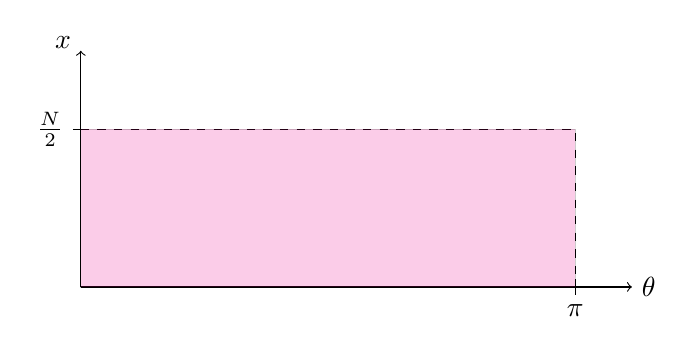
\begin{tikzpicture}
\draw[->] (0,0) -- (7,0);
\draw[->] (0,0) -- (0,3);
\node[below] at (6.28, -0.1) {$\pi$};
\draw (-0.1,2) -- (0.1,2);
\draw (6.28, -0.1) -- (6.28,0.1);
\node[left] at (-0.1, 2) {$\frac{N}{2}$};
%\addplot[blue, domain = 0:6.28, samples = 201] {sin(x)};
\draw[dashed] (0,2) -- (6.28, 2) -- (6.28,0);
%\draw[blue, domain=0:6.28] plot (\x, {2*sin(0.5*\x r)});
\draw [fill=magenta, opacity= 0.2] (0,0) rectangle (6.28, 2);
\node [right] at (7, 0) {$\theta$};
\node[left] at (0, 3.1) {$x$};
\end{tikzpicture}

\end{center}

This shaded region represents all possible configurations of the needle. Try it yourself! Pick a point in the rectangle and draw what the needle looks like at that point. For example, picking a point and random and eye-balling the location of the needle:

\begin{minipage}{0.5\textwidth}
\begin{flushleft}
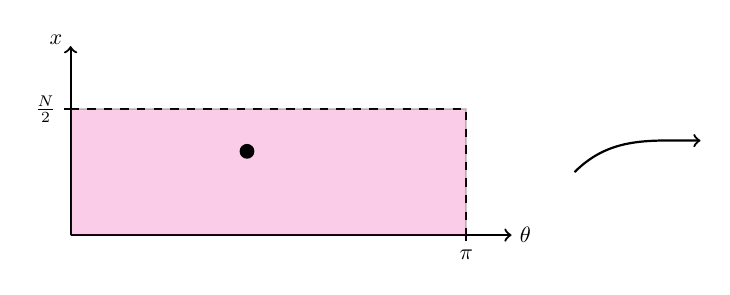
\begin{tikzpicture}[thick,scale=0.8, every node/.style={scale=0.8}]
\draw[->] (0,0) -- (7,0);
\draw[->] (0,0) -- (0,3);
\node[below] at (6.28, -0.1) {$\pi$};
\draw (-0.1,2) -- (0.1,2);
\draw (6.28, -0.1) -- (6.28,0.1);
\node[left] at (-0.1, 2) {$\frac{N}{2}$};
%\addplot[blue, domain = 0:6.28, samples = 201] {sin(x)};
\draw[dashed] (0,2) -- (6.28, 2) -- (6.28,0);
%\draw[blue, domain=0:6.28] plot (\x, {2*sin(0.5*\x r)});
\draw [fill=magenta, opacity= 0.2] (0,0) rectangle (6.28, 2);
\node [right] at (7, 0) {$\theta$};
\node[left] at (0, 3.1) {$x$};
\draw[->, thick] (8, 1) to [out =45, in = 180] (10,1.5);
\node[fill=black,draw=black,circle,inner sep=2pt] at (2.8,1.33) {};
%\draw[dashed] (0, 1.33) -- (2.8, 1.33) -- (2.8, 0);
\end{tikzpicture}
\end{flushleft}
\end{minipage}
\begin{minipage}{0.5\textwidth}
\begin{center}
\includegraphics[scale=0.35]{Bouffon6}
\end{center}
\end{minipage}

You can see in the picture that the dot is located around $\frac{2}{3}$ of the way up the box and about halfway across. This corresponds exactly to the pictured needle, which is similarly close to the walls and rotated almost half a turn (i.e. slightly less than $90^{\circ}$). 

The question is now this: in our probability space, how do we represent the set of all configurations that touch or cross the walls? \hypertarget{cross} Is there some sort of formula, perhaps a function of $x$ and $\theta$, that will tell us when the needle touches the wall and when it doesn't?\footnote{Justin Timberlake actually \href{http://www.youtube.com/watch?v=iVzmPeSCQMM}{wrote a song about this}, believe it or not \hyperlink{cross}{\textbf{\textcolor{red}{$\uparrow$}}}}

It turns out that yes, we can! Take a look at these pictures and see if you can figure it out. 
\begin{figure}[h]
\begin{minipage}{0.3\textwidth}
\centering
\vspace{-0.25cm}
\includegraphics[width=\textwidth]{Bouffon7}
\caption{Fully Crossing}
\end{minipage}
\begin{minipage}{0.3\textwidth}
\centering
\includegraphics[width=\textwidth]{Bouffon8}
\caption{On The Wall}
\end{minipage}
\begin{minipage}{0.3\textwidth}
\centering
\vspace{-0.1cm}
\includegraphics[width=\textwidth]{Bouffon9}
\caption{Not Crossing}
\end{minipage}
\end{figure}

Think about those pictures for a second. Can you see any sort of formula in terms of $x$ and $\theta$ that might describe the cases in which the needle touches/crosses the wall? Let me direct your attention to another feature of this needle diagram, which I will label $\mathbf{A}$. It's the vertical line that runs from the tip of needle to the height of the center of the needle. Pics or it didn't happen:

\begin{figure}[h]
\begin{minipage}{0.3\textwidth}
\centering
\vspace{-0.25cm}
\includegraphics[width=\textwidth]{Bouffon10}
\caption{Fully Crossing\\ \vspace{-0.5cm}$$A > x$$}
\end{minipage}
\begin{minipage}{0.3\textwidth}
\centering
\includegraphics[width=\textwidth]{Bouffon11}
\caption{On The Wall\\\vspace{-0.5cm} $$A = x$$}
\end{minipage}
\begin{minipage}{0.3\textwidth}
\centering
\vspace{0.1cm}
\includegraphics[width=\textwidth]{Bouffon12}
\caption{Not Crossing\\ \vspace{-0.5cm}$$A < x$$}
\end{minipage}
\end{figure}

Well how 'bout that! We now have an inequality that states explicitly when the needle touches or crosses the wall: when $A \geq x$. If we can obtain a formula for $A$ in terms of $\theta$, then we can actually plot this relationship on the rectangular grid of all possible configurations. Take a gander at this:
\begin{align*}
\sin{(\theta)} &= \frac{\text{Opposite}}{\text{Hypotenuse}} \\
\sin{(\theta)} &= \frac{A}{^N\!/_2} \\
\implies A &= \frac{N}{2}\sin{(\theta)}
\end{align*}

So, in other words, the needle crosses or touches the line whenever:

$$A \geq x \Longleftrightarrow x \leq \frac{N}{2}\sin{(\theta)}$$

And now I can actually graph this! Check it out. Here's the graph of $x = \frac{N}{2}\sin{(\theta)}$:

\begin{center}

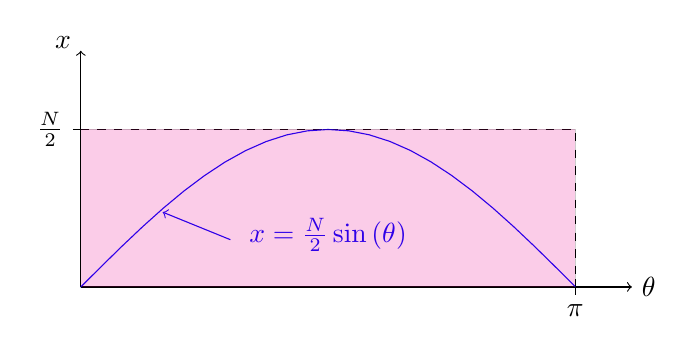
\begin{tikzpicture}
\draw[->] (0,0) -- (7,0);
\draw[->] (0,0) -- (0,3);
\node[below] at (6.28, -0.1) {$\pi$};
\draw (-0.1,2) -- (0.1,2);
\draw (6.28, -0.1) -- (6.28,0.1);
\node[left] at (-0.1, 2) {$\frac{N}{2}$};
%\addplot[blue, domain = 0:6.28, samples = 201] {sin(x)};
\draw[dashed] (0,2) -- (6.28, 2) -- (6.28,0);
\draw[blue, domain=0:6.28] plot (\x, {2*sin(0.5*\x r)});
\node[below, blue] at (3.14, 1) {$x = \frac{N}{2}\sin{(\theta)}$};
\draw [->, blue] (1.9, 0.6) -- (1.04, 0.95) ;
\draw [fill=magenta, opacity= 0.2] (0,0) rectangle (6.28, 2);
\node [right] at (7, 0) {$\theta$};
\node[left] at (0, 3.1) {$x$};
\end{tikzpicture}
\end{center}

So if I want the parts where $x \leq \frac{N}{2}\sin{(\theta)}$, all I have to do is shade in the part underneath the curve:
\begin{center}
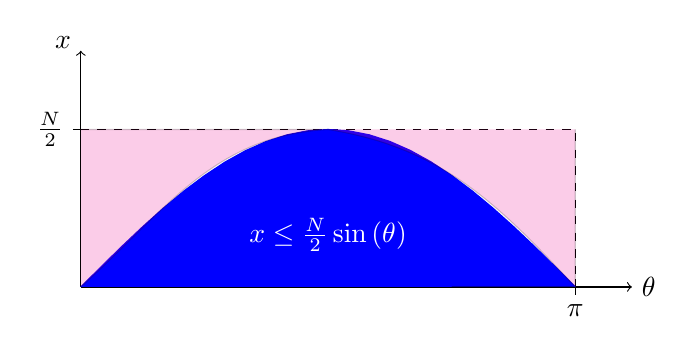
\begin{tikzpicture}
\draw[->] (0,0) -- (7,0);
\draw[->] (0,0) -- (0,3);
\node[below] at (6.28, -0.1) {$\pi$};
\draw (-0.1,2) -- (0.1,2);
\draw (6.28, -0.1) -- (6.28,0.1);
\node[left] at (-0.1, 2) {$\frac{N}{2}$};
%\addplot[blue, domain = 0:6.28, samples = 201] {sin(x)};
\draw[dashed] (0,2) -- (6.28, 2) -- (6.28,0);
\draw[blue, fill=blue, domain=0:6.28] plot (\x, {2*sin(0.5*\x r)});
\node[below, white] at (3.14, 1) {$x \leq \frac{N}{2}\sin{(\theta)}$};
%\draw [->, blue] (1.9, 0.6) -- (1.04, 0.95) ;
\draw [fill=magenta, opacity= 0] (0,0) rectangle (6.28, 2);
%\draw[fill = magenta, opacity = 0.2, domain=0:6.28] plot (\x, {(1-sin(0.5*\x r)});
\draw[fill = magenta, opacity = 0.2] (0,0) to [out = 42, in = 183] (3.14,2) -- (0, 2);
\draw[fill = magenta, opacity = 0.2] (3.14,2) to [out = -9, in = 133] (6.28,0) -- (6.28, 2);
\node [right] at (7, 0) {$\theta$};
\node[left] at (0, 3.1) {$x$};
\end{tikzpicture}
\end{center}

Nice! We can now clearly see when the needle is and is not crossing the walls. The big rectangle represents all possible needle configurations, and the blue hump represents all those which touch/cross the wall. But remember the original question we're trying to ask: what's the probability that a randomly tossed needle will touch the line?

To answer this question, let's think a little bit about what a probability actually is. If you, like me, ask the question ``what is the probability that I will marry Beyonc\'{e}?" you must consider the small (but not completely insignificant!) part you play in all of the universe's Beyonc\'{e} suitors. That probability would then look something like $\frac{\text{My Beyonc\'{e} seduction}}{\text{The world's Beyonc\'{e} seduction}}$. Basically, when you think about probability, you think about the frequency of the desired event relative to the total landscape of all possible results. For that reason, the probability of flipping heads is $\frac{1}{2}$, since heads is one option out of the possible two, and rolling any given number on a die is $\frac{1}{6}$. 

Looking back at our question, it's worth remembering that this is a question of \textit{geometric probability}. So, in this case, the space of all possible outcomes is the $\pi \times \frac{N}{2}$ rectangle. It's our job to figure out what proportion of that rectangle is made up of cases in which the needle touches or crosses a line. In other words, we need to figure out:

$$P(\text{crossing line}) = \frac{\text{Area of Blue Part}}{\text{Area of Rectangle}}$$

\hypertarget{civil}Well, the denominator is a breeze. The area of the rectangle is just $\frac{N}{2}\pi$. The area of the blue part, however, requires a li'l bit of integration.\footnote{Integration is key. This next bit of math is dedicated to the Civil Rights Movement \hyperlink{civil}{\textbf{\textcolor{red}{$\uparrow$}}}}

\begin{align*}
\text{Area of Blue Part} &= \int_0^\pi \frac{N}{2}\sin(\theta)\;\text{d}\theta \\
&= -\frac{N}{2}\cos(\theta)\Bigr\rvert_{\theta = 0}^{\theta = \pi}\\
&= -\frac{N}{2}(\cos(\pi) - \cos(0))\\
&= \frac{N}{2}(\cos(0)-\cos(\pi))\\
&= \frac{N}{2}(1 - (-1))\\
&= \frac{N}{2}\cdot 2\\
&= N
\end{align*}

Interesting! It turns out the area of the blue curve is exactly equal to the length of the needle. We're now ready to find the probability:

\begin{align*}
P(\text{crossing line}) &= \frac{\text{Area of Blue Part}}{\text{Area of Rectangle}}\\
P(\text{crossing line}) &= \frac{\cancel{N}}{\frac{\cancel{N}}{2}\pi} \\
P(\text{crossing line}) &= \frac{2}{\pi}
\end{align*}

Sweet!! That's a pretty awesome result. The probability of a randomly tossed needle crossing the line is exactly $\frac{2}{\pi} \approx 65\%$. Perhaps more awesome, though, is this rearrangement of the equation:

$$\pi = \frac{2}{P(\text{crossing line})}.$$

What does this mean? It means that the next time you're bored, you should sit tossing a needle onto equally spaced parallel lines for a few hours. Count the proportion of tosses that cross a line, then take 2 divided by that number. Believe it or not, you'll be left with one hella accurate approximation to $\pi$.  

Take a second to appreciate how REDONKULOUS this is. We can find a reasonably accurate value for $\pi$, this seemingly enigmatic constant whose value has eluded mathematicians for thousands of years, by simply tossing some sticks onto the floor. I guess that all it took to figure this out was that puffy shirt. Good work, Bouffon. 

There's actually a whole branch of computer programs that use exactly this kind of technique to make numerical approximations. The idea is that randomness can somehow provide novel insights and make some calculations easier. They're called Monte Carlo methods, and are named after the casino at which their inventor's uncle would often gamble away the family fortune (fo realz! I'm not making this stuff up). 

\begin{figure}[h]
\centering
\includegraphics[scale=0.4]{MonteCarlo}
\caption{A Scenery That Says ``Let's Work On Numerical Approximation Algorithms!"}
\centering
\end{figure}
The idea behind Monte Carlo approximations is really simple. Say you want to calculate the area of a circle, can't remember the damn formula, but happen to have at your disposal a very efficient way of generating thousands of random numbers. I know that I find myself in this situation probably twice a week. You can do something similar to Bouffon's method and drop a couple bajillion points into a square that around your circle. Here's a picture:

\begin{figure}[h]
\centering
\includegraphics[scale=0.5]{MonteCarlo2}
\caption{Dots 'n' Stuff}
\centering
\end{figure}

If a point is dropped at random into this box, what are the odds of it falls into the quarter-circle? Well, it's simply the proportion of box that the circle occupies. Since it's a $1 \times 1$ box, this part of the circle has area $\frac{1}{4}\pi (1)^2 = \frac{\pi}{4}$. So all you gotta do is count the proportion of points that have fallen into the circle, multiply it by $4$ and you're golden! Another fantastic approximation for $\pi$. Monte Carlo methods are exceptionally powerful and are used by just about every computer out there. 

Before I finish this section, I should probably remind you that if you wanna see how Bouffon's needle works when the needle is shorter than the width of the floor, check out \hyperref{AppendixB}{Appendix B}. If you're looking for another revelatory, ground-breaking result, you'll probably be kind of disappointed; the method is almost identical for the case we just did and the solution ends up being pretty similar too. It's still probably worth taking a quick peek!
\end{comment}

\begin{comment}
\section*{Art Inspired By $\pi$}
\addcontentsline{toc}{section}{Art Inspired By $\pi$}

I've seen a couple of cool pieces of art based on $\pi$. If I wanted to be a total jerk, I could just show you a pictures of art that has lots of circles and say that it contains $\pi$. You'd probably feel pretty cheated. So I'm going to veer away from that and actually show you some artwork that's inspired by the \textit{digits of $\pi$}. I first discovered these images through  \href{http://www.youtube.com/watch?v=NPoj8lk9Fo4}{a Numberphile video}, which will tell you in visuals everything I'm about to tell you in writing, so if you would prefer that maybe it's just best to watch the video. It's ok. I won't be upset.\vspace{\bigskipamount}

You're still here! I'm flattered.\hypertarget{smith} Let's look at some $3.14$ ins$\pi$red art. Most of these pictured were created by a fella named Martin Krzywinski, with some help from his buddy\footnote{I'm just guessing his collaborator was his friend. It's possible they were actually enemies but had a Mr. \& Mrs. Smith kind of relationship \hyperlink{smith}{\textbf{\textcolor{red}{$\uparrow$}}}} Cristian Vasile. More of their stuff can be \href{http://mkweb.bcgsc.ca/pi/art/}{found here}. The dudes have made some pretty cool stuff!

Here's the first one:

\begin{figure}[h]
\centering
\includegraphics[scale=0.55]{PiArt1}
\caption{Stare At It For 30 Seconds And You'll See Jesus}
\end{figure}

Each circle represents a different digit of $\pi$. The border of the circle represents the ``current" digit, while the inside of the dot is the next digit. \hypertarget{hope}So, you can see that the second and fourth dots have the same outside (since they represent $3.\mathbf{1}4\mathbf{1}\ldots$), while the first and third have the same inside.\footnote{``But aren't we all the same coloured dots on the inside?" you say, timidly but with a glimmer of hope. ``Yes, yes we are," I reply, as we ride together on our majestic stallions into the night \footnotemark}\footnotetext{Warning: this is the prompt for my next book. Stay tuned for that one!\footnotemark} \footnotetext{Yo, look how meta these embedded footnotes are. I could keep this going forever. But I won't. Back to the art! \hyperlink{hope}{\textbf{\textcolor{red}{$\uparrow$}}}} It's a very beautiful picture! What it does really well is illustrate the incredible power of randomness within $\pi$. There doesn't seem to be any discernible pattern, and even if you stare at some curious group of dots for a while your attention is quickly shifted to another place on the page. 

As a number, it's suspected that $\pi$ is what's called \textit{normal}, which is a horrible jargon term for a number as strange as this one. The idea is pretty simply: a number is normal if it's infinite decimal expansion is completely random. In other words, every digit is equally likely to appear at any time. The picture above nicely illustrates the apparent normality of $\pi$.	Regardless, it's a fantastic visualization and speaks volumes about the strong interplay between math and art.\vspace{\bigskipamount}

The second $\pi$ picture is kinda unreal if I do say so myself. Here's how it works. You starts off with a picture of the 9 digits arranged in a circle, with each digit getting a different colour, like this:
\begin{figure}[h]
\centering
\includegraphics[scale=0.7]{PiArt2}
\end{figure}

You start the drawing on $3$, the first digit of $\pi$. You then jump across the circle to $1$, then $4$, then back to $1$, and so on. You keep on tracing out the digits of $\pi$ in this way, changing the colour of the lines depending on the colour associated with each number. When all is said and done, you end up with a picture so spectacular it can't even fit on this page.\label{text} \hyperref[PiArt]{Go check it out on top of the next page} then come back here. Take your time and fully absorb its beauty!

\begin{figure}[h]
\centering
\includegraphics[scale=0.45]{PiArt3}
\caption{Pi Art Or Grandma's Next Needlepoint Project?\label{PiArt} \\ \hyperref[text]{Head back up!}}
\end{figure} 
Welcome back! That was awesome, right? Go take another look. It's that cool. So how does that work? Well, every ``transition" between  numbers is presumably completely random. So, there should theoretically be an equal distribution of ``1-step" jumps, ``2-steps," and so on. This picture is a good indication that this is true, and in fact you can clearly see the distinct patterns that each jump pattern makes. For example, at the center of the image, around the picture of the $\pi$, you can see that there are $5$ distinct jumps that go all the way across the circle, and together they form a pentagon shape. The fact that each side of that pentagon is equally think means that each of those transitions is equally likely. 
\begin{wrapfigure}{r}{0.3\textwidth}
\centering
\vspace{-0.55cm}
\includegraphics[scale=0.4]{LineCurve}
\caption{Just Imagine What It'd Look Like On Shrooms!}

\end{wrapfigure}
The coolest part is that these random patterns end up forming clear shapes within the diagram. For example, there's the illusion of perfectly formed circles radiating outward from the center. There are no actual circles, since every line in the picture is going from one number-spot to another, but it's actually surprisingly easy to make a bunch of crossing straight lines look like they're curved. Check out the picture on the right! Plus, the fact that there end up being circles in a picture of $\pi$ is wicked. \\

One last thing: I can't show GIFs in this document, but there's a pretty sweet GIF that illustrates how this picture was made. It's an incredibly spend-up time lapse of the picture being constructed, and it's well worth the 3 seconds. \href{http://i.kinja-img.com/gawker-media/image/upload/s--Oee8L243--/pi9axtfeevhr5or9s4qi.gif}{Here is is}.
 \vspace{\bigskipamount}

Here's a third $\pi$ visualization. \hypertarget{baby}This one's pretty tricky to get at first, but once you see the trick it's pretty breathtaking.\footnote{\href{http://www.youtube.com/watch?v=CwEXAJZ-y7A}{And I use that term pretty loosely} \hyperlink{baby}{\textbf{\textcolor{red}{$\uparrow$}}}}
\begin{figure}[h!]
\centering
\includegraphics[scale=0.37]{PiPrank}
\caption{A Creative Visualization Of A Transcendental Number}
\end{figure}

Psych. That's a picture of polka dots. \hypertarget{whimsy}I obtained it by Googling ``polka dots." You were hopefully totally fooled.\footnote{Was it an act of malice? \href{https://screen.yahoo.com/maya-rudolph-snl-skits/maya-angelou-prank-show-000000680.html}{No, it was an act of whimsy} \hyperlink{hope}{\textbf{\textcolor{red}{$\uparrow$}}}}\vspace{\bigskipamount}

Here's another awesome picture. \hypertarget{spiral}Once again, each digit is given a different colour, but this time they're put into a spiral. 
\begin{figure}[h]
\centering
\includegraphics[scale=0.18]{PiArt4}
\caption{Are The Dots Moving?!?\protect\footnotemark}
\end{figure}

\footnotetext{No \hyperlink{spiral}{\textbf{\textcolor{red}{$\uparrow$}}}}

There are around $3500$ digits pictured here, and there's actually a feature of $\pi$ that we can see in this illustration that we haven't been able to see yet. It's called the \textbf{Feynman Point}, named after the legendary physicist Richard Feynman. The ``point" is actually a sequence of six $9$s in the digits of $\pi$, which occur starting at the $762$nd spot. It's named after Feynman because he once said that he should memorize the digits of $\pi$ up to that spot, so he could recite them and cleverly finish with ``nine, nine, nine, nine, nine, nine, and so on." See if you can spot it on the spiral picture! First figure out which colour corresponds to the digit nine, then see if you can find six of them in a row. If you can't find them they're circled on the picture atop the next page. 


\begin{figure}
\centering
\includegraphics[scale=0.2]{PiArt5}
\end{figure}

But why should we limit ourselves to only $3500$ points in the spiral? By making the dots super tiny, there's no reason we can't include tens, or even hundreds of thousands of points. Here's what that looks like:

\begin{figure}[h]
\centering
\includegraphics[scale=0.3]{PiArt6}
\caption{Yeah, These Are Really Just Random Pictures Of Colours At This Point}
\end{figure}

The fact that the third of those, which is veering into over $100 000$ digits, looks like a pretty uniform blob, is another indication that $\pi$ is a truly random number. 
\end{comment}


{\Large \textcolor{Plum}{Well there you have it! A sneak preview of my book about $\pi$, which I hope to have completed in September. I hope you learned something and had a good chuckle in the process. Thanks for taking a look!}} 
\vspace{2cm}
\begin{figure}[h]
\centering
\includegraphics[scale=0.6]{Obama}
\end{figure}


\begin{comment}
\section*{Conclusion}

Well, there you have it! Thus ends our journey through with $\pi$. We started way back in Egypt and Babylon, made our way to Greece with Archimedes, took a tour of Europe and Asia with some famous approximations, and then found a few wonky places where $\pi$ shows up completely unexpectedly. You're now equipped with an understanding of why $\frac{1}{\sqrt{2\pi}}$ shows up in the bell curve, you know the dimensions of King Solomon's pool, and you know how to approximate $\pi$ by throwing sticks on a tiled floor. 

I can't thank you enough for reading through this whole thing and making it all the way here. You're a champion. Here's a virtual hug. You deserve it!





\newpage
\section*{Appendix A: Derivation of the Normal Distribution}
\addcontentsline{toc}{section}{Appendix A: Derivation of Normal Distribution}

\newpage
\section*{Appendix B: Bouffon's Needle for $D>N$}\label{AppendixB}
\addcontentsline{toc}{section}{Additional Solution To Bouffon's Needle}

\end{comment}

\end{document}




